\documentclass{article}
\usepackage{fullpage}
\usepackage{graphicx}
\usepackage{../svn-multi}

\title{Thinking in Proto}
\author{By Kathryn McGuire, Jacob Beal, and other authors of MIT Proto}
\date{Last Updated: \today}

\newcommand\code[1]{\begin{center}\var{#1}\end{center}}
\newcommand\problem[1]{\begin{quote}{\em #1}\end{quote}}

% arguments/keystrokes:
\newcommand\var[1]{{\tt #1}}
\newcommand\qvar[1]{``{\tt #1}''}
\newcommand\key[1]{{\bf #1}}

\usepackage{wrapfig}
\usepackage{subfigure}

\begin{document}

\maketitle

Relax, and don't panic.  You've found {\bf Thinking in Proto}, a
tutorial designed to get you started and demystify the language.
Proto is very different from most other programming languages.  For
most people, even once they've started writing Proto code, it's a big
jump to change how you're thinking and really take advantage of
Proto's continuous space/time model.  This tutorial will hopefully
help you make that jump.

\tableofcontents

% standard LaTeX credits insert; should echo AUTHORS

\section{Credits for Proto}

The Proto language was created in partnership by Jonathan Bachrach and
Jacob Beal.  As they created the language, Jonathan created the first
implementation of MIT Proto, including the first compiler, kernel,
simulator, and embedded device implementations.  Since that time, Jake
and other contributors have built on the work begun by Jonathan.

MIT Proto also includes contributions from (alphabetically):
%
Aaron Adler, Geoffrey Bays, Anna Derbakova, Nelson Elhage, Takeshi
Fujiwara, Tony Grue, Joshua Horowitz, Tom Hsu, Kanak Kshetri, Prakash
Manghwani, Dustin Mitchell, Omar Mysore, Maciej Pacula, Hayes Raffle,
Dany Qumsiyeh, Omari Stephens, Mark Tobenkin, Ray Tomlinson, Kyle
Usbeck, Dan Vickery

The Protobo platform code in platforms/protobo/ also includes 
Topobo-related code from (alphabetically):
%
  Mike Fleder, Limor Fried, Josh Lifton, Laura Yip



\section{How to Use This Tutorial}
	
In writing this tutorial, we have made several assumptions about you
as a reader.  First, we assume you are, if not entirely new to
programming, entirely new to lisp-like languages and many basic
programming statements.  If this is not true, and you have worked with
lisp-based languages, you will find much of the first sections in this
tutorial are easily completed.  We encourage you, however, to read the
``Using The Proto Simulator'' section carefully, as this will be
entirely new, and to read the other sections, paying close attention
to changes in format from the other languages you may have used.
Realize also that though Proto may be similar to other languages, the
way of thinking that must be used by Proto programmers is considerably
different.  Proto allows its user to look at both the individual
devices separately, and at the group of devices as a whole.  For this
reason, we strongly suggest you read the whole tutorial and perform
several of the exercises at the end of each section to strengthen your
learning.

Second, this tutorial is angled towards programmers using the Ubuntu
operating system.  Other Unix or MacOS X users should have no problem,
as they also use terminal in the same way.  Windows users need to
write commands in the command-line prompt on their computer, but the
commands should also work in the same manner.

Finally, we assume that you have installed the Proto Simulator and
compiler.  If you have not, read the information on installing Proto
in the {\bf README} file in the Proto distribution.  If you have
somehow gotten this tutorial without getting a copy of Proto, you can
download Proto from the website: {\tt
  http://stpg.csail.mit.edu/downloads.php}.  This tutorial is based
off of the Release 2, from 11-11-09.  The folder from this download is
essential throughout this tutorial.


\section{Beginning Proto}

Spatial computing is a rapidly expanding field of technology.  A {\bf
  spatial computer} is a collection of computational devices
distributed through physical space, in which the difficulty of moving
information between any two devices is strongly dependent on the
distance between them, and the ``functional goals'' of the system are
generally defined in terms of the system's spatial structure.  Most
programming languages are stretched from their original purposes and
inefficient when applied to meet the needs of spatial computing.
{\bf Proto}, however, is specificially designed for programming spatial
computers.  When trying to program these spatially-embedded systems,
it is hard for programmers to work with each device as an individual,
and try to figure out how those individual actions combine together.
Instead, it is much easier to work with these devices as a whole.
Proto is a great way to do this, because rather than taking this space
as a problem to work around, it embraces the space as something to
take advantage of while programming.  If you want to learn more about
spatial computing in general, one good source is the web site {\tt
  http://www.spatial-computing.org/doku.php?id=scw09:start}.

Proto is a {\bf purely functional language}.  This means that it uses
variables in a mathematical sense and excludes destructive
modifications of data: any identifier refers to an unalterable,
persistent value.  Expressions in Proto are able to be applied to
numerous collections of devices over fields of space.  A Proto user
can use these expressions to perform tasks involving space, time, and
movement, both within the MIT Proto simulator and on devices in the
real world.

This tutorial uses the MIT Proto Simulator to illustrate all of its
program examples.  The Proto simulator takes a statement written into
terminal, compiles it, and runs it on a simulated spatial
computer.  The basic form of a Proto statement written in terminal is:
\code{proto -arguments "(expressions)"}
Let's test this out.  First, go into a
terminal or another command prompt (depending on your operating
system).  Change the directory until you are inside the Proto folder
(use the \qvar{cd} command).  Then run the most primitive program one can,
typing into the {\bf prompt\$} of your terminal:
\code{proto "0"}
It may not seem very exciting, but the dark screen
with little red dots you have in front of you is your first Proto
program.  What's happening?  The \qvar{proto} command reads Proto arguments
from the terminal and summons an assortment of devices in the Proto
simulator.  The \qvar{0} tells Proto that all of these devices are set to
the value 0.  The simulator is not directed to display this value, so
each device is shown as a simple red point, indicating where it is in
space.  The next section covers how to use the simulator.

Open the Proto folder.  Look for a folder inside labeled ``man.''  The
other PDF files inside this folder ({\bf Proto Quick Start}, {\bf
  Proto Language Reference}, {\bf Proto Simulator User Manual}, and
{\bf MIT Proto Developers Guide}) will prove extremely helpful in this
tutorial.  Be sure to keep track of these and use them when necessary.


\section{Using The Proto Simulator}

All right, you easily executed that little basic program earlier.  Now
let's change it up a little.  Take that same program you wrote before
and add a \qvar{-v} before the \qvar{0}.  Your line in terminal should
look like this:

\code{{\bf prompt\$} proto -v "0"}

When you run this, the value of 0 is displayed atop the points in blue
text.  Pull up the {\bf Proto Simulator User Manual}. In this manual
are all of the many arguments that you can put in before the
expressions to manipulate the simulator display.  You can use more
than one argument, and some arguments (\qvar{-n}, \qvar{-r}, etc.) will
take an integer after the argument to change its value.  Without these
arguments, their values are set to the default.  Try this command:

\code{proto -T -n 300 -c "0"}

Now you see a green web that ties together all of the points. You will
notice if you skim the simulator manual and find the \qvar{-c}
argument on page 10 that this argument directs the simulator to
display the green network of communication between devices.  The
\qvar{-T} is what shows the lavender clocks that tick away unevenly at
the bottom of the screen.  The right one keeps track of the speed of
simulation, and the left one displays a count of simulated
``seconds.''  Why is it not displaying real seconds?  This clock runs
at the same speed that the computer is able to process information to
run the simulator.  If the computer is given more information to
process, the clock will run at a slower pace.  Note that these
arguments are case sensitive.  Putting \qvar{-t} here will do
something else entirely.  The \qvar{-n} argument tells the simulator
the number of devices the user wants to work with. \qvar{-n 300}
directs the simulator that instead of the default 100 devices, we want
300.  Execute this again without the \qvar{-n 300}.  The network
becomes much sparser and the time runs much quicker, because there are
less devices to connect and less connections between devices, and
therefore less information to process.  If the \qvar{-n} argument is
not used, the simulator resorts to the default of 100 devices.

\problem{Try this small quiz: add arguments so as to display a network
  of 10 devices with connections between all of them and their values
  displayed as 7.  Then check your answer below.  Hint: this uses one
  argument we have not used yet.}

When you think you have it, look here for our answer. Your
code probably looks something like this:

\code{proto -v -n 10 -c "7"}

If it does, you have this down pretty well.  However, you might be
frustrated with the fact that only a few, or maybe none, of your
points are connected to each other.  If so, the argument you missed
was \qvar{-r}, which sets the distance over which each device can
radio to other devices.  The devices did not connect because they were
too far away from one another to communicate over their short
radio-range.  Execute this code again, and then press ``r'' while in
the simulator. You should see dim gray circles around your devices.
These show how far these devices are communicating. With the \qvar{-r}
command line argument unused, the default radio range is fifteen
meters.  Change the range of radio transmission by adding \qvar{-r
  100} to your list of arguments in the terminal.  Re-execute.  Now
all of your points should be connected to one another.

As we have shown by pressing the ``r'' to show the radio's
transmission range, the simulator can be manipulated inside itself as
well as at the command line.  Many arguments can be switched on and
off, points may be moved, and the simulator can be navigated using the
mouse and keyboard efficiently from within the simulator.

The {\bf Proto Simulator User Manual} document shows many of the ways
that we can manipulate the Proto simulator.  Run the program you just
built again in the Proto simulator. Press ``n.''  The values go away.
If you press ``n'' again they come back.  Leave them off for now.
Press ``c'' and the network also goes away.  Press ``T'' (that's
``shift-t,''---remember, it is case sensitive).  The timer shows up at
the bottom of the screen.  Pressing ``f'' toggles the full screen
mode.  Now turn the network back on, the timer off, and exit full
screen.  Left-click on the screen, and drag the mouse.  The screen
rotates with the mouse.  If you right-click drag, you can zoom in and
out.  To pan, use the arrow keys.  Warning: if you pan after you have
rotated the picture significantly, the directions may be switched
around.  Use ``z'' to reset the view.

Using the Proto simulator manual, try this: make a field of just five
points with values of zero and make the \qvar{-r} range default 15 (or
just do not use \qvar{-r} argument) and display any connections
between the points.  Your code should look like this:

\code{proto -n 5 -c "0"}

Now use the simulator manual to move all these points so that they are
connected. Hint: If you can not find the correct way to move points,
try some of the mouse commands on page 4 of the simulator manual.
Make sure caps lock is off when manipulating the simulator.

\begin{wrapfigure}{R}{0.4\textwidth}
  \vspace{-0.8cm}
  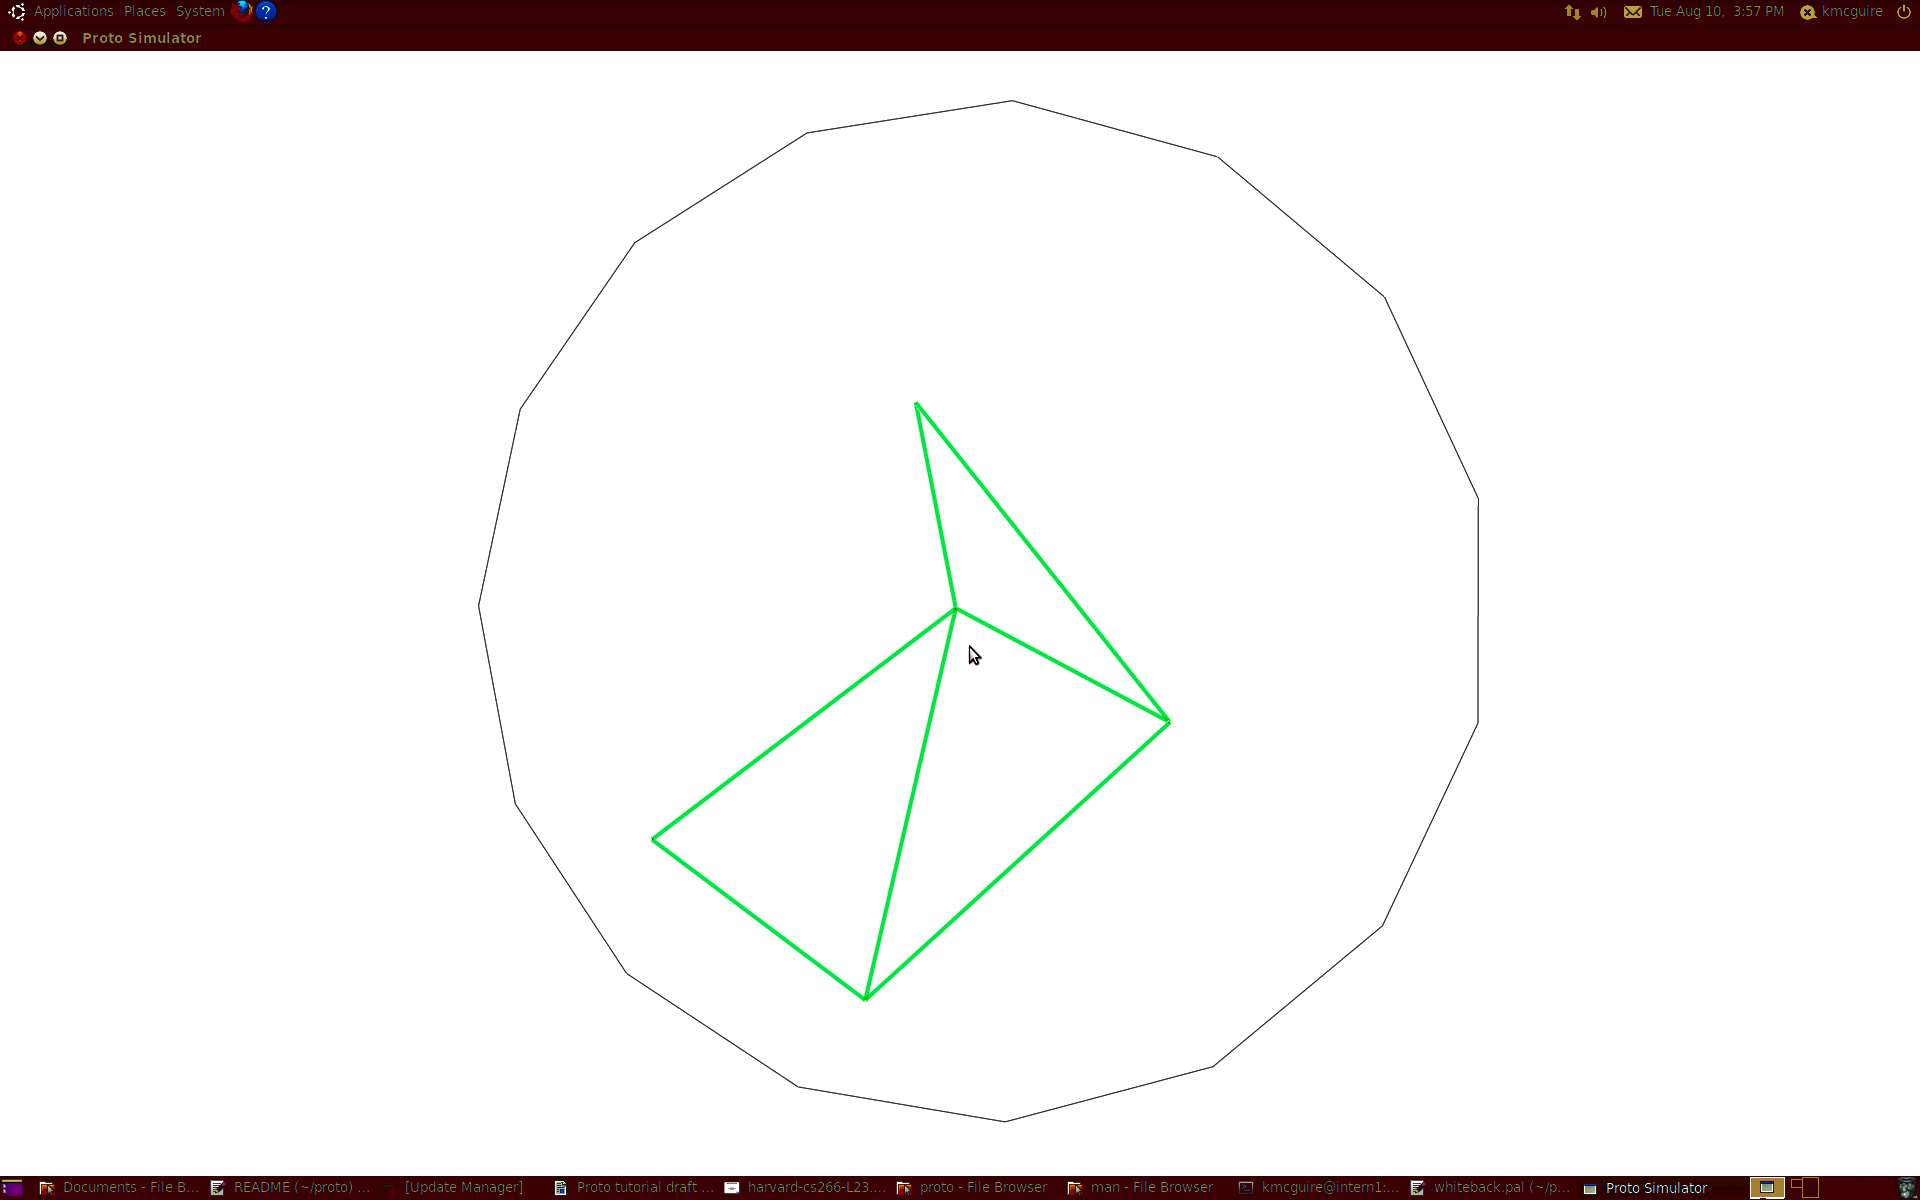
\includegraphics[width=0.38\textwidth]{figures/five-points.png}
  \caption{Five connected devices.}
  \vspace{-0.5cm}
  \label{f:fivepoints}
\end{wrapfigure}

Notice that the green connections latch on to nearby points as you
move a device (Figure~\ref{f:fivepoints}).  (In all the pictures in
this tutorial, the simulator is displayed with a white background for
better printing.  Look in the simulator manual under ``Palette Files''
to find out how to do it yourself.)

Also in the simulator, one can engage three different user test
sensors in a device. This way, one can use \qvar{sense 1}, \qvar{sense
  2} and \qvar{sense 3} points to perform separate actions in a
program.  For now, lets work on just turning them on and off.  Run the
original program again:

\code{proto "0"}

Now, click on a point to select the device. Press ``t.'' Remember:
case sensitive.  It turns the little red dot into a vibrant orange
circle.  You have just turned \qvar{sense 1} on for this point.  Press
``t'' again to turn it off.  Press ``y'' or ``u'' to turn \qvar{sense
  2} or \qvar{sense 3} on.  You can even turn more than one sense in a
single device, and if you shift-left-click-drag you can select and
toggle more than one device at once.  Play around with this to get used
to turning these senses on.  You have now mastered the basics of the
Proto simulator.  Use the Proto simulator manual to explore more.  Many
of the listed arguments we have not yet used will be used later when
writing more advanced functions and expressions.  Try some of these
exercises to enhance your understanding:

\paragraph{Exercises}

\problem{Exercise 1: Execute a program, adding arguments to the
  terminal statement so that the little red points will not be
  displayed and instead only their values will be displayed.}

\problem{Exercise 2: Execute the same, but do not put any arguments in
  the terminal code. Instead, toggle these arguments from within
  simulator. Then kill off three points in the simulator.}

\problem{Exercise 3: Run a network of 1000 devices. Now run them again
  with half the expected number of neighbors (there are several ways
  to do this) and with each simulation step being 0.2 seconds rather
  than 0.01 seconds (there are ways to speed up the simulator).}

\section{The Basics}

Now that we have a strong hold the Proto simulator, let's move on to
the primary part of the command: the expression. Remember the basic
format: \var{proto -arguments "(expression)"} Proto uses the
expression to execute the main tasks of a program.  Even with just the
\qvar{0} there, Proto knows to turn all the devices' values to zero.
Of course, it is going to get far more complicated than a simple zero.
Let's say we want some lucky points we select to be at value one,
while the others remain at zero.

One of the ways we can do this is add an \var{if} expression.  Look up
an \var{if} expression in the {\bf Proto Language Reference}.  This
can be found in your Proto folder in the folder ``man.''  Following
the format, let's build a program that asks if \qvar{sense 1} is
turned on, and if it is, have those points' values be one, and the
other points' values be zero.  It should end up looking like this:

\code{proto -v "(if (sense 1) 1 0)"}

Now the program runs and whenever we turn \qvar{sense 1} on (select a
point and press ``t''), the value of that device becomes 1.  This
works fine, but what if this program was longer, and/or we knew we
might use it multiple times?  In such cases, we define the function in
a separate place and then call on it from the command line.  Create a
new folder for your own programs inside the Proto folder.  I will
refer to this folder as the ``MyPrograms'' folder.  Now go into a
simple text editor, (one that preferably does not use spell check or
auto-correct), and save a new blank document as \var{check.proto}
inside your new folder.  Now that you have somewhere to write your
program, let's create it.

Firstly, we have to define the function.  Look at page 3 in the {\bf
  Proto Language Reference}; there is a explanation beginning with
\qvar{(def}.  This shows the reader how to define a function.
Following the format, start with \qvar{(def check} so ``check'' is the
function name, and then give the function its arguments.  In this
case, we should give it a single argument, \var{src}, which will
designate our source region (in the above case, any point at which
\qvar{sense 1} was true).  These arguments allow Proto to take several
things as input to a function.  In this case, we want it to take
whether a device has \var{(sense 1)} on as its input argument, and store
that information in the local variable \var{src}. So our function definition
could be \code{(def check (src) (if src 0 1))}

Save this code in the text editor, and then go back to terminal.  Make
sure you change directories into your new folder.  The simulator will
only search for functions that are in terminal's current
folder\footnote{The simulator has an argument that can cause it to
  search other places as well.  Look if up and see how.}  Then, we can
simply call the function by saying:

\code{proto -v "(check (sense 1))"}

It works the same way as before, so what makes this so different from
the earlier code?  Well, if this program were a lot longer and you
wrote it out every time in your terminal, it would not be very
efficient for the user at all.  By writing programs in separate
documents, you can not only call functions multiple times, but you can
call functions inside of functions, and in this case, change the
\var{src} of your function to apply it in different cases.  This way,
you could put inside those parentheses after \var{check} in the
terminal call anything that identifies a set of devices, such as any
of the senses, a value, or a function which returns a value.

These \var{if} statements, other than asking if \qvar{sense 1} or any
of the senses are true (non-zero), can also use {\bf logical
  operators} and {\bf conditional statements}.  Logical operators are
used to compare two values in a conditional statement to return a
boolean value (true or false).  In Proto, like in lisp-based
languages, these operators and the numeric operations come before the
values in the statements.  For example, if we want to ask whether
\var{x} is greater than \var{y} we must put the \qvar{>} symbol
before the variables, like so: \code{(if (> x y))}  Similarly, if we
wanted to ask whether \var{x – 1} is still greater than \var{y}:
\code{(if (> (- x 1) y))} With some functions (multiplication,
addition, etc.), the number of arguments after the operators can vary.
Make sure you remember this when you write statements.  Because of the
difference between \var{mux} and \var{if} (described later in the
tutorial, in Section~\ref{s:mux}), there are regular \var{and}s and
\var{or}s, and \var{muxand}s and \var{muxor}s.  The descriptions of
these are all in the Proto Language Reference.  Again, these
\var{and}s and \var{or}s go before their values.

When using logical operators, make sure all the values that you use
are of the same data type.  The many data types are listed on page 2
of the Proto Language Reference.  For now, we will not have to worry
too much about these.  Know, however, that the senses return boolean
values: either true or false.

\problem{Lets try a quick test: Make a function in which if any of the senses
are turned on on a device, that device's LED turns green.}

You may be thinking {\em ``hold up, LEDs?''}.  LEDs are commonly used
as a debugging tool on spatial computers, since we can look at a lot
of devices at once and see an overall pattern.  The Proto simulator
has the ability to turn on or off simulated LEDs for any or all of the
devices in it.  Not all devices have LEDs, though, so the function we
are going to use is {\bf platform specific}, meaning that it comes
from the particular spatial computer we're running on rather than
being universally build into the language.  Many of the sensors and
actuators that we will use are like this.  In this case, we are using
functions the come from running on the simulator, so they are listed
in the Proto simulator manual instead of the language reference.

To turn on an LED, as listed on the bottom of page 9 of the simulator
manual, write one of the three colors of the LEDs (red, blue or
green), and follow it with an intensity level (This level can also be
shown as a physical height above the device).

Go back to your program, \var{check.proto}, and change the \var{1} to
\var{(red 1)}.  It should look like this: \code{(def check (src) (if
  src (red 1) 0))}.  Now go back to terminal and run check again.
Now, when you turn \qvar{sense 1} on at a point, its value does not
change to 1, but instead it has a red LED above it.  No?  That's
because in order to display LEDs, you need a new argument before the
expression.  Replace the \qvar{-v} with a \var{-l} (lowercase l),
since there is not much use for displaying values in this example.
This \qvar{-l} argument tells the simulator to enable LED
display. Your statement in terminal should now look like this:

\code{proto -l "(check (sense 1))"}

Run the program again. Now when you turn on \qvar{sense 1}, a little
red LED turns on above the device.  You can also toggle these LEDs on
and off by pressing uppercase ``L'' from inside the simulator.  You
can turn on multiple \qvar{sense 1}s and get the red LEDs at more
devices.

\problem{Now retry the test from above.  Hint: The \var{or} operator
  comes in handy.  If you are stumped, or if you think you have done
  it correctly, the solution is below.}

\begin{wrapfigure}{r}{0.4\textwidth}
  \vspace{-0.8cm}
  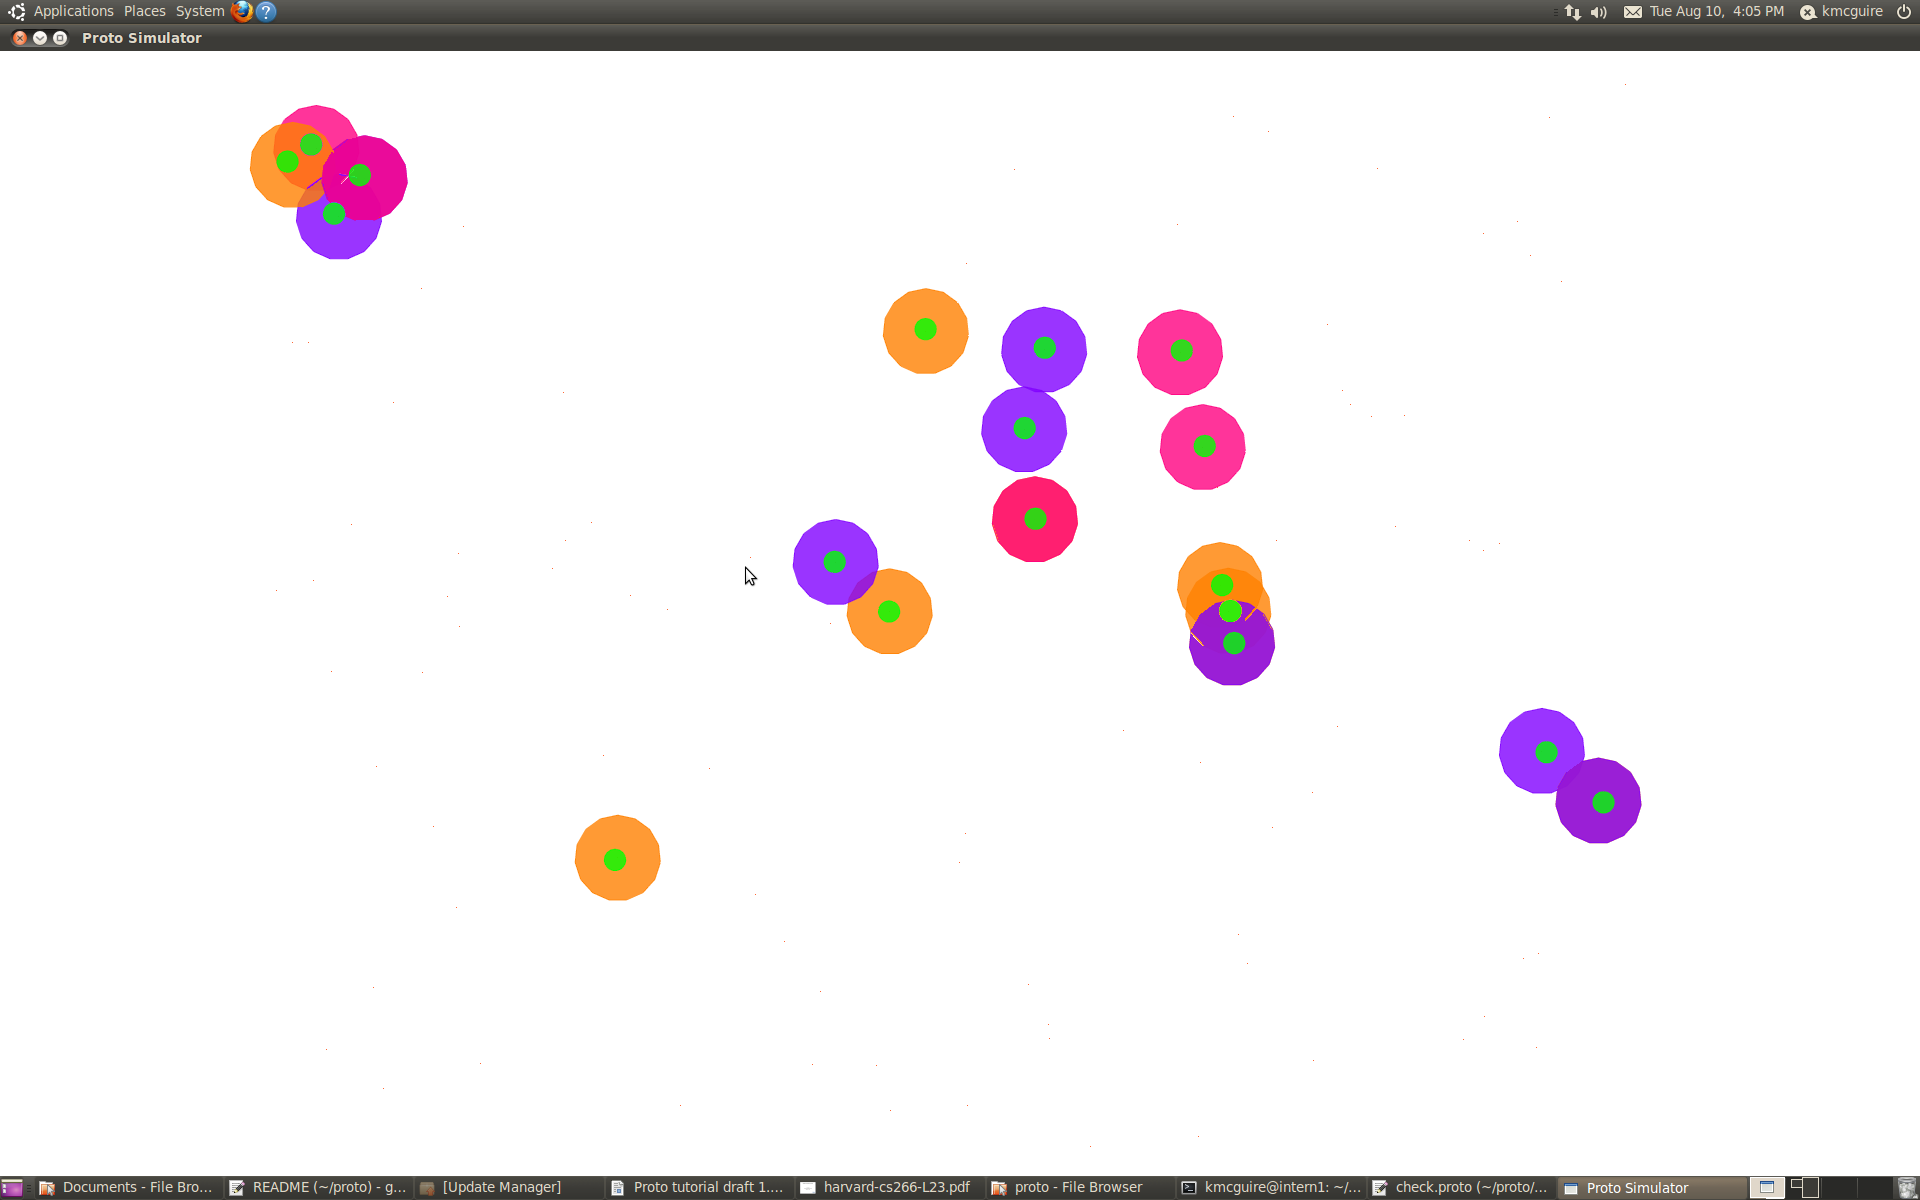
\includegraphics[width=0.38\textwidth]{figures/sense-led.png}
  \caption{Green LEDs wherever a \qvar{sense} is turned on.}
  \vspace{-0.5cm}
  \label{f:leds}
\end{wrapfigure}

In fact, you do not even have to change functions for this program.
Just change your \qvar{(red 1)} to \qvar{(green 1)} in
\var{check.proto}, and save the text.  Then run \var{check.proto}, but
change the \var{src} you give into the function from terminal from
\qvar{sense 1} to include all three senses.  You can include all three
by using the \var{or} operator.  The \var{or} operator can only take
two values after it, but we can nest the \var{or}s, so that it takes
all three senses into account.  {\bf Nesting} is a common practice in
Proto, as with other programming languages.  Nesting is the practice
of placing a function call inside another function call.  Nested
\var{or}, \var{if} and \var{mux} statements will be common in
Proto.\footnote{Note that Proto is expected to have a multi-input
  \var{or} statement an upcoming release.}  Your statement in the
terminal should look similar to this:

\code{proto -l "(check (or (sense 1) (or (sense 2) (sense 3))))"}

If you run this and turn on a few \qvar{sense 1}s, \qvar{sense 2}s,
and \qvar{sense 3}s (keys ``t,'' ``y,'' and ``u''), you should end up
with several multicolored circles in your simulator, each wth a green
circle at the center (Figure~\ref{f:leds}).  If the program is not
working check these things:

\begin{itemize}
\item Did you remember to save \var{check.proto} when you had
  finished? If not, terminals still running the older version of your
  program. Make sure that the file name ends in ``.proto,'' or else it
  will not be recognized as a Proto file.
\item Does your code look like this: \qvar{(def check (src) (if src
    (green 1) 0))}?
\item Are you in the correct directory in terminal: inside Proto and
  inside the programs folder where \var{check.proto} is saved?
\item If the simulator exits with a ``segmentation fault'' error, it
  usually means you have one too few or one too many parentheses
  somewhere.  Even parentheses around the 0 at the end of the function
  will cause this error, because it makes Proto think that 0 is
  supposed to be a function rather than a number.  In more advanced
  functions, it may mean a misconstruction of a \var{let} or other
  syntactic construct.
\item Is there anything besides your code in the \var{check.proto}
  file? The Proto simulator will try to interpret any regular text as
  Proto code unless it is commented out (covered later).
\end{itemize}

Once you get this running, congratulations! You have grasped the
basics of Proto. In the next chapters we will move on to how we can
manipulate three different aspects of Proto: space, time, and
movement, in order to succeed in more advanced functions.

\paragraph{Exercises}

\problem{Exercise 1: Tell the devices to turn on different LEDs based
  on what senses are turned on.}

\problem{Exercise 2: Tell all devices to turn on red LEDs, except if
  any sense is turned on, in which case return different values (2, 3,
  4) based on what sense is turned on.}

\problem{Exercise 3: Turn on a red LED only on a device that has ALL
  of the senses turned on on it.}


\section{Using Space}
\label{s:space}

Space is easy to manipulate in Proto, because Proto was designed for
devices to work together by sending signals across space to other
devices.  Take a look at this code:

\begin{quote}
\begin{verbatim}
(def close (src) 
  (let ((d (distance-to src)))
    (if (and (< d 3) (> d 1)) 
      (blue 1) 
      (blue 0))))
\end{verbatim}
\end{quote}

There are several new things in this code. For instance, the \var{let}
(which you surely recognize if you have used lisp programming before).
This \var{let} assigns the variables inside it to new values.  In this
\var{let} statement, \var{d} is set as the distance to the source.
The function \var{distance-to}, as its name suggests, gives each
device its own value of estimated distance to the source.  You can
look up these functions in further detail in the Proto Language
Reference.  Put this program into a new blank text document and save
it into your programs folder as \var{close.proto}. Call it with this
in your terminal:

\code{proto -l -n 1000 "(close (sense 1))"}

Remember that \qvar{-n} sets the number of devices, which means this
program has 1000 devices to work with. Now \var{src} is set to
\var{(sense 1)}, so if we execute this program, and turn on
\qvar{sense 1} for a few devices, you will see that only devices
within a very small select range from the \var{src} turn on their blue
LED.  If you turn on \qvar{sense 1} on a fairly isolated device, you
might not have any of the surrounding device LEDs turn blue at all.
The program tells each device to figure out their distance to the
\qvar{sense 1} device, which they should call \var{d}, and that if
their individual value of \var{d} is less than three meters and
greater than one meter, then they may turn their LEDs blue.
Otherwise, the LEDs remain blank \var{(blue 0)}.  Try expanding this
range of blue LEDs by increasing the first parameter of the \var{and}
statement (remember to save and re-execute your code to try the
program).

This is all good and fine, but what if we wanted to be more precise in
our selection?  What if, instead of taking three points or no points,
based on how close the randomly placed points were to the src, we
wanted just a single closest point, no matter how far or close it is
to the src?  This is where the \var{nbr} and the \qvar{hood} functions
come in.  These functions are used to tell a device exactly where each
point within its communication range is relative to itself and what
values these neighbors have calculated, giving the device fields of
points and values to work with. Using these functions, we can select
the point(s) that we want accurately. This function demonstrates that:

\begin{quote}
\begin{verbatim}
(def closest (src) 
  (let ((d (distance-to src)) 
        (min-d (broadcast src (min-hood+ (nbr (distance-to src)))))) 
    (if (and (not (= min-d (inf))) 
             (= min-d d)) 
      (blue 1)
      (blue 0))))
\end{verbatim}
\end{quote}

This code is built to light up the device LED that is closest to the
\var{src} (source) blue, and it introduces a wide variety of new
functions.  Let's walk through how to make it, step by step.  First,
create a file called \var{closest.proto} inside your folder in the
Proto directory.  Inside that, define the function \var{closest} as a
function that takes argument \var{src}.

We see our \var{let} function again, except this time it defines two
separate variables instead of just one.  The first one we know
already: variable \var{d} is the distance to the source device. The
second definition is where most of the confusing bit comes in.

We are trying to assign the value of the shortest distance to the
source to our new variable \var{min-d} (minimum distance).  Let's work
from the inside parentheses out in this definition.  First, we have
our \var{distance-to src}.  Note that you cannot use the predefined
\var{d} here, because \var{let} defines everything at once, and so
Proto will not recognize this variable as being already defined.
Later, we will cover how to use the \var{let*} function to
sequentially define variables.  Now that each device has established its
own distance value (which happens to be the same as \var{d}).  The
\var{nbr} function gathers up these values from each device's
neighborhood, returning a field that maps each point in the
neighborhood to a distance value.  All the functions starting with
\var{nbr} in the Proto Language Reference create fields of values
assigned to neighboring devices.  In fact, instead of putting
\var{(nbr (distance-to src))} here, one could instead put
\var{(nbr-range)}, which again assigns a field of distances to
neighbors, with the same outcome since for this program we only care
about neighbors of the \var{src}.  The \var{min-hood+} function takes
all of these values returned by \var{nbr} as pairs, (neighbor,
distance away), and then takes the minimum ``distance away'' value as
its return value.  This is important: because of the \qvar{+} at the end
of \var{min-hood}, the device chooses to ignore the value that it
itself gives.  

\begin{figure}[ht]
  \centering
  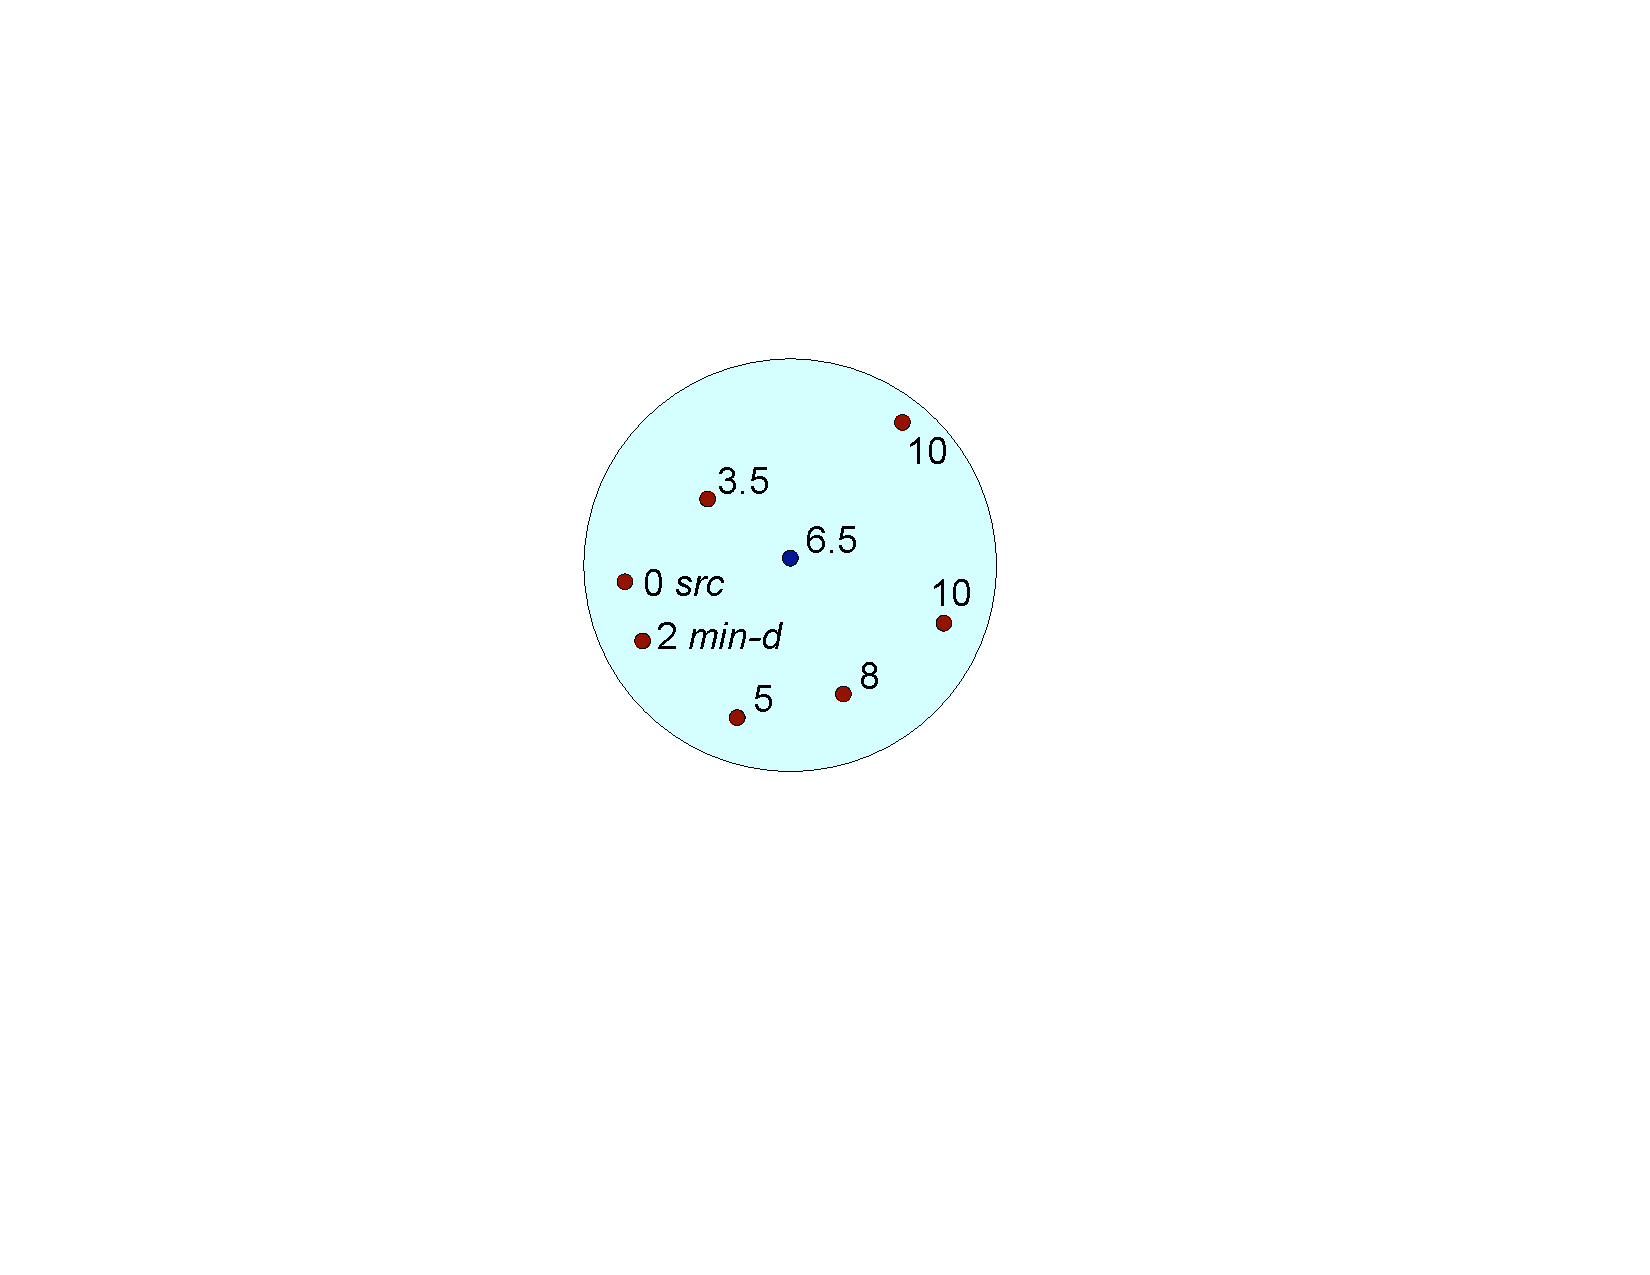
\includegraphics[width=0.4\textwidth]{figures/nbr-d.pdf}
  \caption{Field of \var{nbr} values of \var{d} for a device (dark
    blue) near a \var{src} device.}
  \label{f:nbrd}
\end{figure}

Were this not the case, the closest device to itself would always be
itself.  If you examine page 11 in the Proto Language Reference,
notice that most of the neighbor summary functions allow for this
\qvar{+} differentiation.  The broadcast function says that every
device must take the value of \var{min-d} from the nearest source
device.  Otherwise, each device's interpretation of variable
\var{min-d} is different depending on what values it gets from the
devices around it.  If there is one source, every device holds the
same \var{min-d} value, that determined by the source device.  The
source device \var{broadcast}s to all of the other devices in the
network that \var{min-d} equals the distance to the source's closest
device.

The main part of this function, (after the \var{let}) is actually
quite simple.  All it does is have each device ask itself, ``Is my
distance to the source equal to the minimum distance to the source,
and is the minimum distance to the source not infinity? If so, turn
LED blue; if not, leave LED blank.''  This part: \var{(not (= min-d
  (inf)))} stops the devices from automatically turning blue, because
before any source is identified, the minimum distance to the source is
infinite, and all the devices' \var{d} variables are also infinite and
therefore equal to \var{min-d}.  This test tells the program to wait
until a \var{src} exists, which will cause \var{min-d} become finite.
Remember that if you want to look over any of the \var{nbr},
\var{hood}, \var{broadcast} or \var{not} functions, or even how to
use constants such as \var{inf}, you can find them all in the Proto
Language Reference.

This is how to call the \var{closest} function in the terminal, much like
the \var{close} function:

\code{proto -l "(closest (sense 1))"}

\begin{wrapfigure}{R}{0.4\textwidth}
%  \vspace{-0.8cm}
  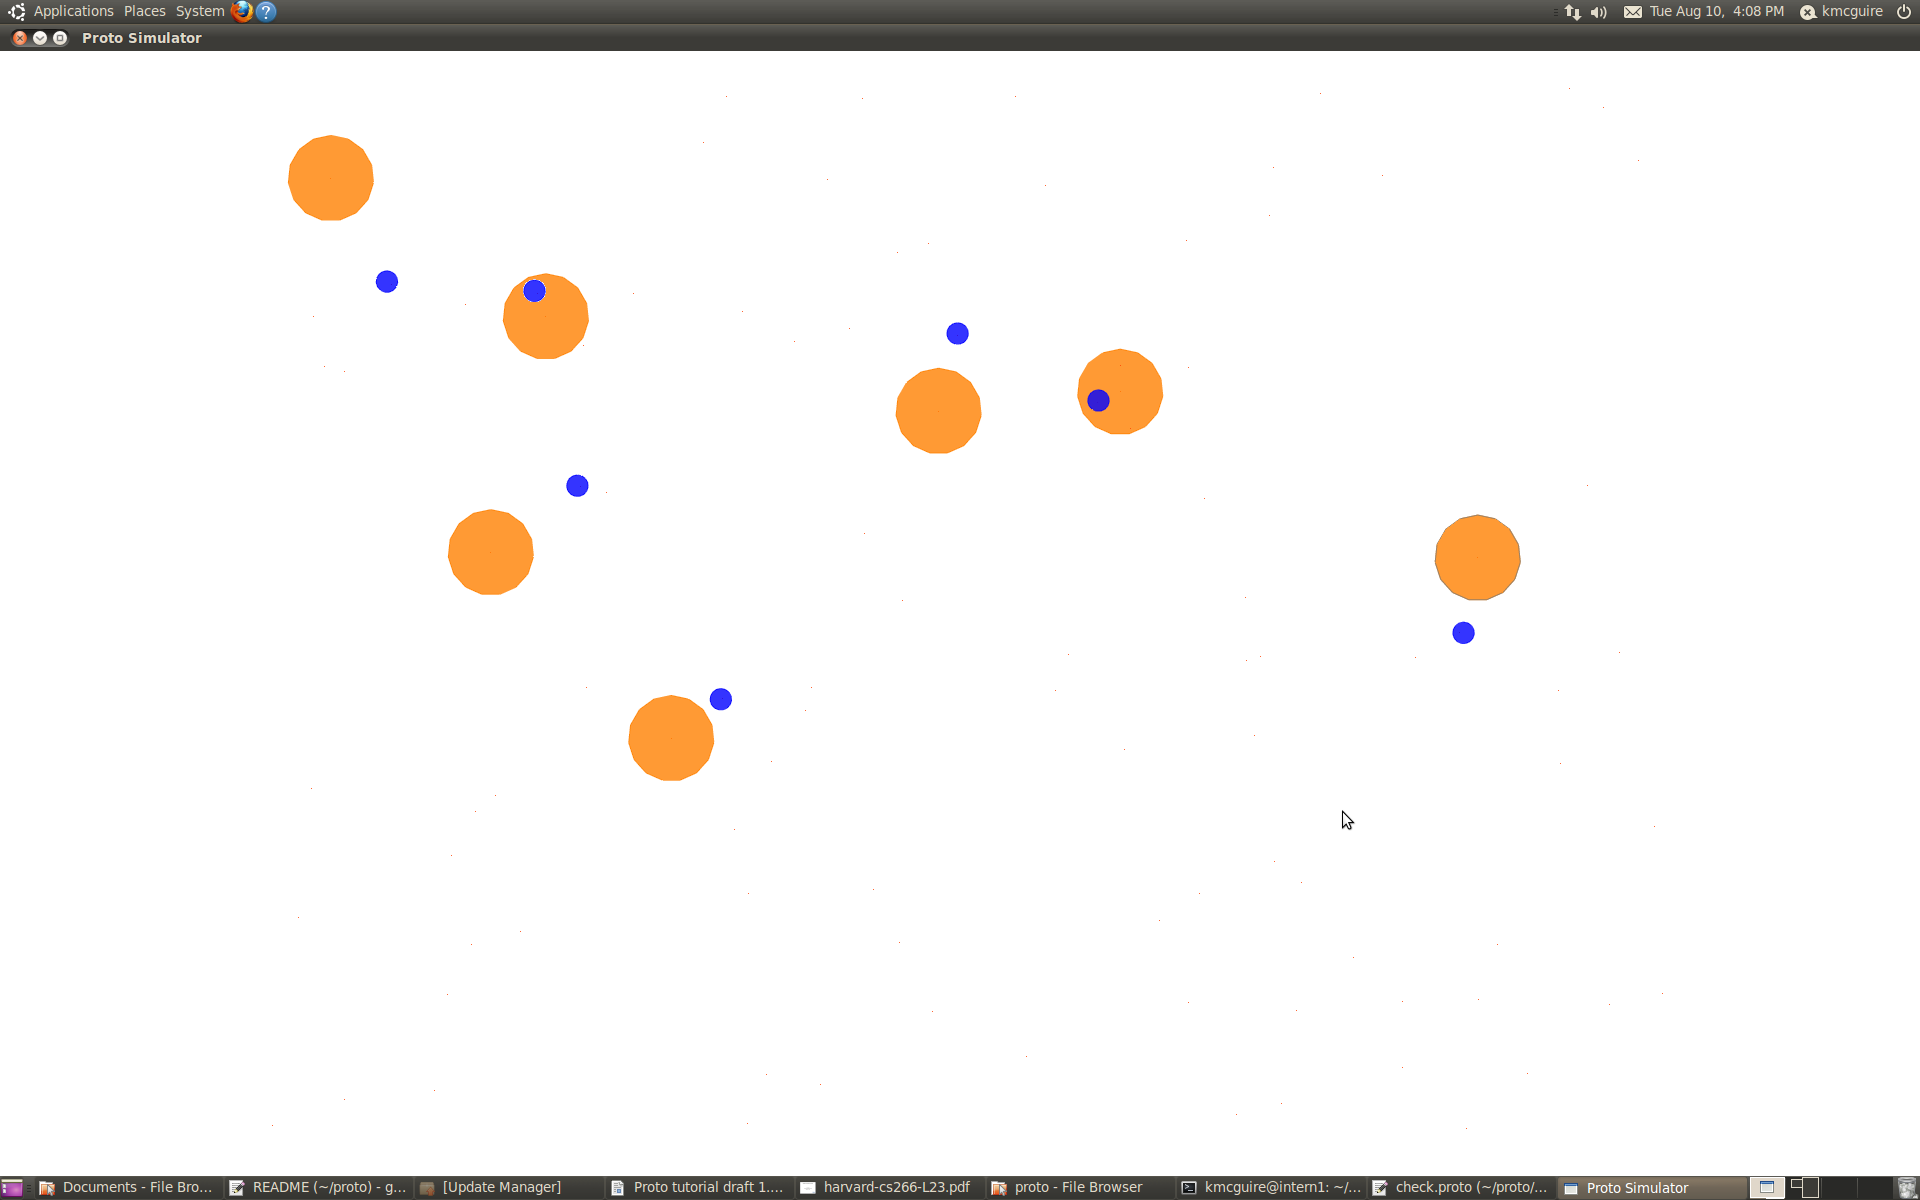
\includegraphics[width=0.38\textwidth]{figures/closest.png}
  \caption{Running the \var{closest} program}
  \vspace{-0.5cm}
  \label{f:closest}
\end{wrapfigure}

When executed, this produces a field of devices, shown as little red
dots.  Right now, all the devices know that \var{min-d} is equal to
infinity, and therefore all their LEDs are off.  Turn \qvar{sense 1}
on on any device.  After a few seconds, a blue LED goes on on the
closest device to the \var{src}, no matter how close or far that
device may be.  You can turn \qvar{sense 1} on or off at several
devices, and their closest neighbors' LEDs will turn on or off
accordingly, since the \var{broadcast} is taking the value from the
{\em nearest} source (Figure~\ref{f:closest}).  Take note, however,
that if you isolate a \qvar{sense 1} device to the point that all
other points are outside of its radio-range, no \var{min-d} can be
found.  Also, turning on two \qvar{sense 1} devices close together may
allow only a single \var{min-d} value (depending on where exactly the
closest neighbors are), so only one of the sensed points may light up
its closest neighbor.  Similarly, if a \qvar{sense 1} device is with
direct communication range of another \qvar{sense 1} device, both will
light their LEDs, since they both see the other being zero distance
from the \var{src}.

\problem{Try this test: Write a program in which all the points create
  a bullseye target-board using LEDs.  You don't have to use any
  \var{nbr}s or \var{hood}s for this program.  Remember to refer to
  the Proto Language Reference whenever you get stuck.  You can do
  this any way you like with any colors you like.  Remember, 100
  points don't create much of a bullseye, so use the \var{-n} argument
  to create more points (1000 points should work well).  If it seems
  complicated, you are probably over-thinking things.  Hint: Nested
  \var{if}s may prove helpful.}

When you're finished, look here for the answer.  Our code, which may
differ from yours some, looks like this:

\begin{quote}
\begin{verbatim}
(def bullseye (src)
  (let ((d (distance-to src)))
    (if (< d 15)
        (red 1)
        (if (and (< d 30) (> d 15))
          (green 1)
          (if (and (< d 45) (> d 30))
            (blue 1)
            0)))))
\end{verbatim}
\end{quote}

and I call it with this command:

\code{proto -n 1000 -l "(bullseye (sense 1))"}

Again, this uses the \var{let} and \var{distance-to} functions, and
sets \var{d} to the \var{(distance-to src)}.  Then each device asks
itself whether it is within 15 units from the source, between 15 and
30 units from the source, or between 30 and 45 units from the source,
and then sets its LED color accordingly.  If it is in none of these
three ranges, no LED will turn on, and it just returns zero.  This
text should again be saved in a file in your folder in Proto, as
\var{{\em itsname}.proto}.  The name of the file before \var{.proto}
should be the same (capitals and everything) as the name of the
function.  So in this case, the file is called \var{bullseye.proto}
and is in your ``MyPrograms'' folder.

\begin{wrapfigure}{R}{0.4\textwidth}
  \vspace{-0.8cm}
  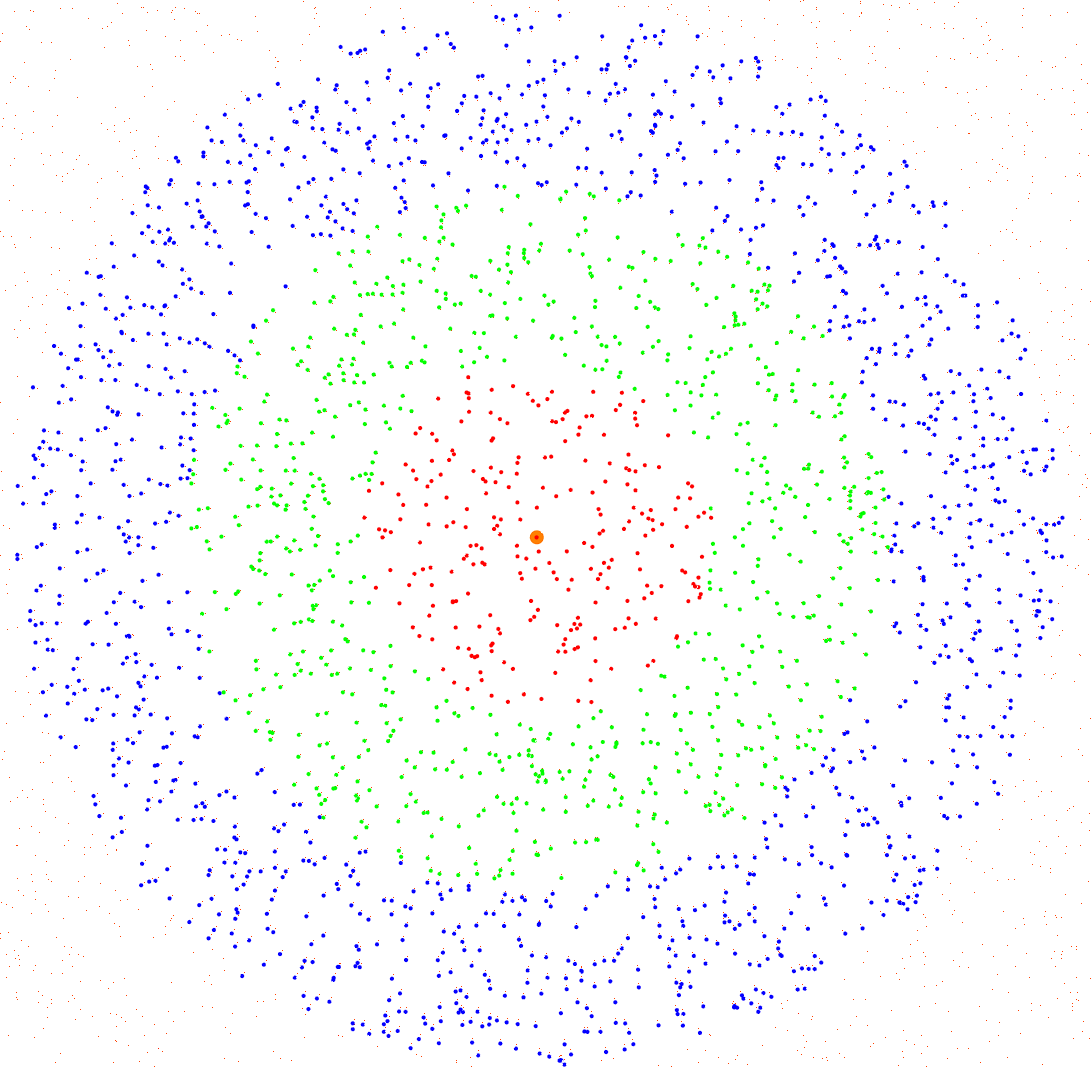
\includegraphics[width=0.38\textwidth]{figures/bullseye.png}
  \caption{Running a \var{bullseye} program}
  \vspace{-0.5cm}
  \label{f:bullseye}
\end{wrapfigure}

To call this program, I changed the number of devices to 1000, so it
could be clearly seen in the Proto simulator.  You can use more
devices, but remember, the more devices you use, the slower your
program begins to run.  After 5000 or so devices, this program works
very slowly, if at all.  You can, however, speed up the simulator with
the \var{-s} argument (find this in the Proto simulator manual).  I
also recommend that you begin saving your terminal call statements
{\em inside} your program text file, so you know how to call the
program in future use.  Just make sure that if you do, you add a “;”
in front of it, which will comment it out so that Proto does not read
it as it is reading the file.  You should do this with anything you
add to your Proto files that you do not want to be executed.  It is
good practice to add descriptions of your code in this way also.  When
this program executes, it fills the simulator with 1000 little red
devices.  When I put a device on \qvar{sense 1} that is approximately
mid-screen, red dots begin to fan out, and then green, and then blue.
Eventually the LEDs form a pretty nice target-board.

One can use these functions using distance, \var{nbr}s and
\var{hoods}, incorporated with movement and time functions to create
all sorts of useful Proto programs involving space.  You now know enough
to create many geometric patterns in Proto.

\paragraph{Exercises}

\problem{Exercise 1: Create a program in which any device that is on
  the shortest path from a \qvar{sense 1} device to a \qvar{sense 2}
  device turns its LED green.}

\problem{Exercise 2: Adjust the previous program so that the points
  within the path also turn their LEDs red if they are close to the
  \qvar{sense 1} or sense \qvar{2 points} (within 5 meters).}

\problem{Exercise 3: Adjust the \qvar{bullseye.proto} program to make
  the LED lights be at a height above the device based on the distance
  to the source. Remember, in \var{(red 1)}, the \var{1} sets a height
  for the LED to be displayed.}

\section{Restricting Space}
\label{s:mux}

When we write a Proto program, we aren't just stuck to using the same
space that we started with.  We can change 

You've already seen the function that will be used to do this.  The
\var{if} function actually works by restricting the space that each of
its two sub-expressions runs in.  For example, try running this
program in your terminal:

\code{proto -l "(if (sense 1) (red 1) (green 1))"}

Anywhere that you turn on \qvar{sense 1}, the red LED turns on and the
green LED does not.  Everywhere that you don't turn on \qvar{sense 1},
the green LED turns on and the red LED does not.  Thought about in
terms of individual devices like this, what is happening is fairly
intuitive.

We can also think about this program in terms how it is acting over
the whole space at once.  In this view, the \var{if} is actually
changing {\em where} the program runs.  Ordinarily, when we write a
piece of Proto code, it runs everywhere at once.  When we wrap a piece
of code in an \var{if}, it splits the space into two parts.  In the
part of space where \qvar{sense 1} is turn on, it runs the program
that turns on the red LED.  In the other part, it runs the program
that turns on the green LED.  This way of thinking about running a
Proto program may be less intuitive, but thinking about it this way
will help to understand more complicated programs.

\begin{figure}[ht]
\centering
\subfigure[]{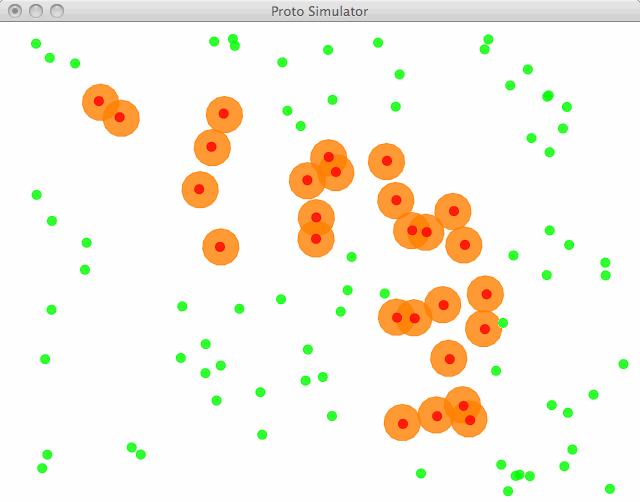
\includegraphics[height=2in]{figures/restrict.png}}
\subfigure[]{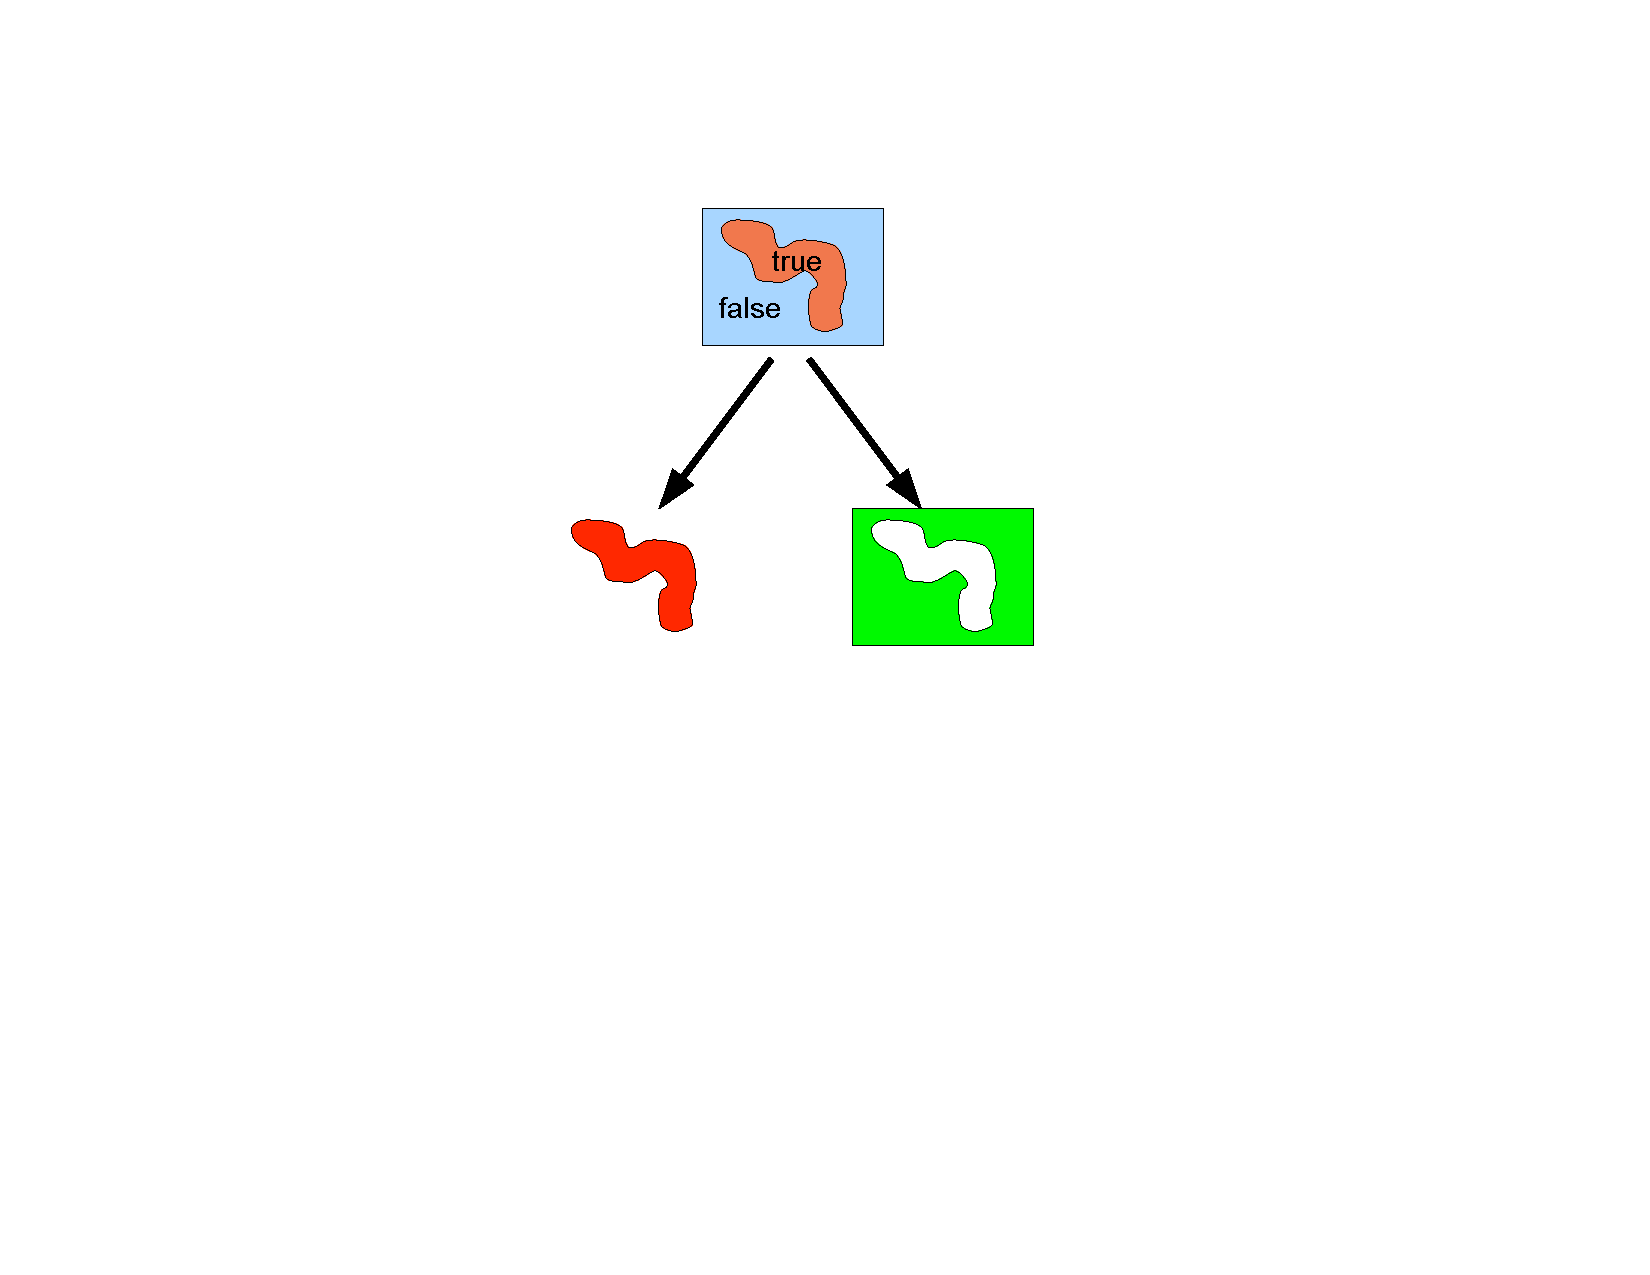
\includegraphics[height=2in]{figures/restriction.pdf}}
\caption{When \var{if} is used to choose which LED to turn on (a), it
  splits the space into two parts and runs each branch only in its own
  part.}
\label{f:restriction}
\end{figure}

Let's use our new understanding to think about how \var{if} should
interact with computations over space.  When we use functions like
\var{distance-to} or \var{broadcast}, they are not doing their
calculations by magic: each of these functions is a computation over
the devices in our space, built out of simpler functions like
\var{nbr} and \var{min-hood}.  This means that changing the space with
an \var{if} will change what the function computes.

Try using your new understanding of how \var{if} changes space
to predict what will happen when you run this program:

\code{proto -l -c "(if (sense 1) 0 (red (< (distance-to (sense 2)) 100)))"}

\begin{wrapfigure}{R}{0.4\textwidth}
  \vspace{-0.8cm}
  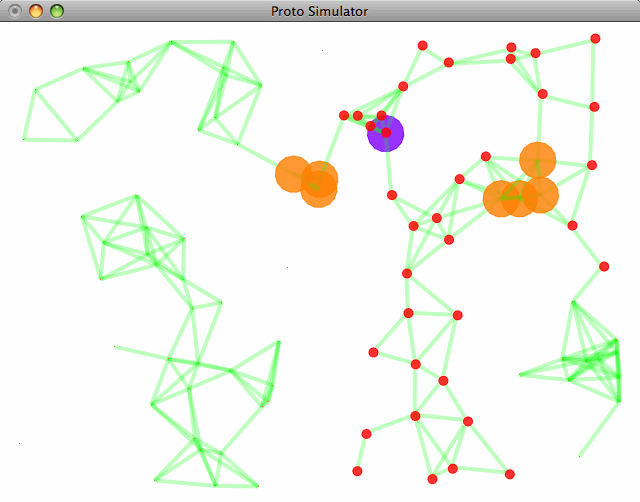
\includegraphics[width=0.38\textwidth]{figures/blocked-distance.png}
  \caption{A \var{distance-to} calculation running restricted to one
    branch of an \var{if}}
  \vspace{-0.5cm}
  \label{f:blockdist}
\end{wrapfigure}

When you run the program, try turning on \qvar{sense 2} at a device
and then turning \qvar{sense 1} on and off for groups of nearby
devices.  Did you guess what would happen?  The \qvar{sense 1} devices
act like blockages, making the distance measurements computed by
\var{distance-to} flow around them.  It's as if those devices aren't
there at all---and because of the \var{if}, that's exactly what
it looks like to the part of the program running \var{distance-to}!

Sometimes we want to be able to split up our space like this, and
sometimes it is a problem.  For example, let's say we want to make our
devices play the ``hot and cold'' guessing game.  A few of the devices
will secretly decide that they are the targets of the guessing game.
We will make a guess by turning on \qvar{sense 1} at a device.  The
device will turn on a green LED if we guessed right, a red LED if
we're close to a target, and a blue LED if we're far away from all the
targets.

Here's some Proto code to implement the ``hot and cold'' game:

\begin{quote}
\begin{verbatim}
(def hotcold ()
  (let ((target (once (< (rnd 0 1) 0.03))))
    (if (sense 1)
      (all (green target)
           (red (< (distance-to target) 25))
           (blue (> (distance-to target) 50)))
      0)))
\end{verbatim}
\end{quote}

All of the functions in this code should be familiar except for
\var{all} and \var{once}.  The \var{all} function takes any number of
expressions and runs them all, then returns the value of the last one.
In this case, we're using it to check whether each of the three LEDs
should be turned on.  The \var{once} function computes its expression
just once, then remembers the value---we'll learn more about how it
can work in the next section.  Here, we're using it to have each
device flip a coin and decide if it's once of the targets.  We do it
with \var{once}, because we don't want the devices to keep flipping
coins and changing their minds.

Put the program in \var{hotcold.proto} and try running it with:

\code{proto -l -c "(hotcold)"}

\begin{figure}[ht]
\centering
\subfigure[Wrong]{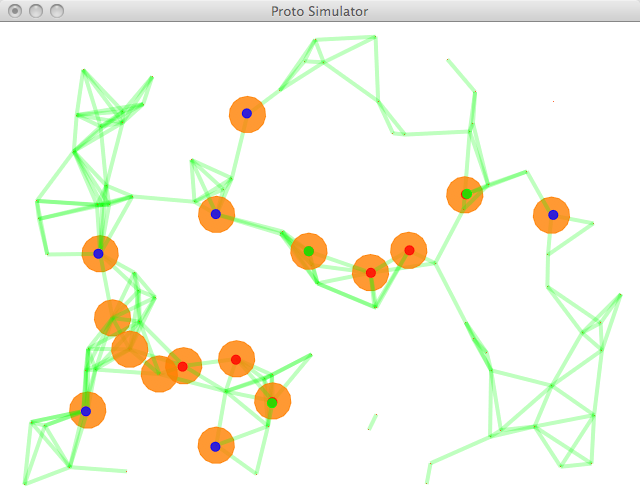
\includegraphics[width=0.4\textwidth]{figures/ifhotcold.png}}
\subfigure[Correct]{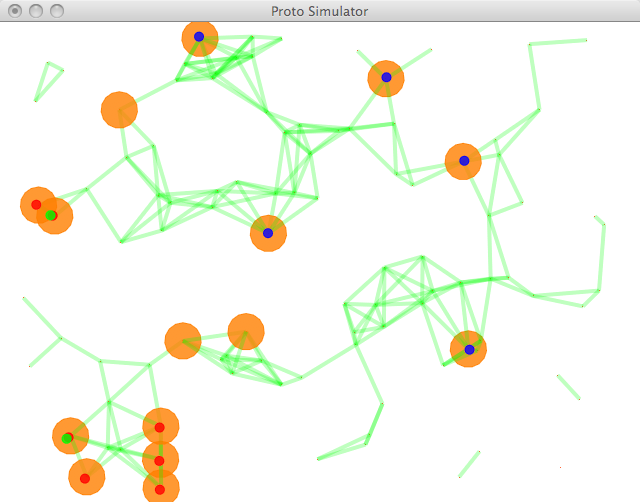
\includegraphics[width=0.4\textwidth]{figures/muxhotcold.png}}
\caption{A ``hot and cold'' game running incorrectly (a) and correctly (b).}
\label{f:ifvmux}
\end{figure}

Do you notice something wrong with how the program is running?  It's
really hard to find the targets!  When you make a guess, it almost
always shows up blue.  In fact, you can't get any to show up red until
after you find a target, and then all of a sudden a whole bunch of
blue LEDs turn red!  And even once you've found a target, the devices
nearby won't necessarily end up with the right colors.  What's
happening here?

You guessed it!  The problem is the \var{if} that we are using.  When
the program branches on \qvar{sense 1}, that is changing the space
where the LED calculations are running.  Rather than running
everywhere, they run only on the devices where we have already made
guesses.  Why is this so bad?  Think about what happens if you guess a
device that's right next to one of the targets.  When we run the
\var{distance-to} function on that device, it uses \var{nbr} and
\var{nbr-range} in order to figure out how far it is from the nearest
target.  You should think about \var{nbr} not just as a device getting
information from its neighbors, but also as {\em sharing} information
with its neighbors.  So if a device isn't in the same branch of an
\var{if}, it won't share its information.  Even though there is a
target right next door, unless we've already guessed the target, the
target won't be sharing information in the \var{distance-to}, and the
device we just guessed at won't be able to tell that it's close.

For this reason, there is another type of branch in Proto.  This
function is called \var{mux}, and it works just like \var{if} except
that both branches run everywhere.  This is a very useful tool for us,
because it lets the two branches share information back and forth if
they want to.  Now, the test expression is used to pick which branch
gives the final value of the functions, rather than picking where each
branch runs.  We need both \var{if} and \var{mux} branches: sometimes
we will want to stop information from flowing and will use \var{if}
and other times we will want to share information and will use
\var{mux}.

\problem{Let's try this out: try rewriting the ``hot and cold'' game
  using \var{mux} instead of \var{if}.}

When you're finished, look here for the answer.  Our code, which may differ
from yours, looks like this:

\begin{quote}
\begin{verbatim}
(def hotcold ()
  (let ((target (once (< (rnd 0 1) 0.03))))
    (green (mux (sense 1) target 0))
    (red (mux (sense 1) (< (distance-to target) 25) 0))
    (blue (mux (sense 1) (> (distance-to target) 50) 0))))
\end{verbatim}
\end{quote}

Try running this version, using the same terminal command as before,
and see that it's now working correctly.  When you tried fixing the
\var{hotcold} program, you might have had a hard time getting the LEDs
to not turn on until you hit \qvar{sense 1}.  If that happened to you,
it's because \var{mux} is running both branches, not just the one that
gets picked in the end.  So if you run \qvar{(mux (sense 1) (red 1)
  (green 1))} you'll always have both the red LED and the green LED
on!

You now understand one of the trickiest bits about thinking in Proto.
When we write our programs, we're not just computing over space, we're
changing the space where we're computing.  If you think carefully
about {\em where} your program is running, you will always be able to
understand what is going on and how to get your programs right.

\paragraph{Exercises}

\problem{Exercise 1: Fix the \var{hotcold} program without using \var{mux}.}

\problem{Exercise 2: Create an ``intersection of bullseyes'' pattern.
  Use two sources, and around each source create a bullseye pattern
  with a radius of 45 meters.  Only turn on LEDs in the overlap
  between two bullseyes overlap, and only turn on the LED for the
  father distance.  When the sources are on top of one another, this
  should produce a perfect bullseye, and when they're barely close
  enough to intersect it should produce a thin perpendicular patch of
  the outermost color.}

\problem{Exercise 3: Calculate how far every device in space is from
  \qvar{sense 1}, if we restrict travel to only those locations within
  20 meters of \qvar{sense 2} and more than 50 meters from \qvar{sense 3}}

\section{Using Time}
\label{s:time}

In Proto, as with any programming language, time is an important part
of its programs.  We have already seen how to display the Proto
simulator's main clock at the bottom of the simulator screen.  This
clock is always running whether or not we choose to display it,
counting how many simulated seconds of time have gone by.  We know
that in Proto, our timers, like this one, will not run in actual
seconds, but will run at whatever rate Proto is managing to run
through its program.\footnote{The simulator has a command line option
  to keep simulator and actual time synchronized.  Can you find it?}

Now we will start working with time directly in our programs as well.
Let's start by setting a simple timer on every device.  Call this
inside your terminal:

\code{proto -v "(rep t 0 (+ t (dt)))"}
	
When it executes, you will see a hundred devices timing things at
various ``second'' lengths.  Some display nine seconds while others
display seven or ten.  They have different values because each device
is running its own independent internal clock, and these clocks are
not necessarily synchronized with one another.  The program is being
run in rounds, once per second, and time it runs its value changes.

To display the discord between devices clearly, run the program again,
this time setting the number of devices to five and changing how much
the devices differ from one another:

\code{proto -v -n 5 -desired-period 0.3 -desired-period-variance 0.1 "(rep t 0 (+ t (dt)))"}

With only five devices, you can more easily watch how the timers run
at different rates.  Turn on the timer at the bottom of the screen
(press capital ``T'' while in the Proto simulator).  Notice that all
the devices' timers still manage to stay with around the same value as
the overall simulator time shown on the bottom-left corner of the
screen.  To see this more clearly, you may want to pause the simulator
and step its time forward in small increments: press ``s'' to step and
``x'' to resume fast execution.

There are a two new functions in here: \var{rep} and \var{dt}.  Both
are defined on page 5 of the Proto Language Reference.  Take a look at
the form of \var{rep}.  The \var{rep} function creates a variable,
just like \var{let}, but the variable created by \var{rep} is used to
remember information from round to round of the program.  In this
case, we use the function \var{rep} to create the feedback variable
\var{t}, which will store elapsed time and has the initial value of 0.
The third argument, \qvar{(+ t (dt))}, tells the how the value changes
over time---how it ``evolves.''  In this case, Proto reads that every
time it runs through this code, it should add one \var{(dt)} to the
current time.  What is one \var{dt}?  This \var{dt} value is the
amount of time elapsed between rounds in a program.  So we essentially
add the time of one round every time we go through a round.  The whole
\var{rep} expression then returns the value of \var{t}.  We can also
make more complicated feedback functions using \var{letfed}, which can
make more than one feedback variable and allows you to use them in a
further part of the program just like variables from a \var{let}.

Let's say our field is a giant field of microwaves.  Do we want our
microwave timer running all the time, and on all the machines?  Of
course not.  Let's try put some limits on our timer.  We only want
this timer to run on the microwaves that are turned on.  Create a file
with this function in a new file in your programs folder:

\begin{quote}
\begin{verbatim}
(def MWTimer (src)
  (if src (rep t 0 (+ t (dt))) 0))
\end{verbatim}
\end{quote}

Make sure that you save it correctly inside the Proto folder. Then run
it from terminal.  Try this call from terminal on your own.  Tell the
simulator to show the values, and put the source in as \qvar{sense 1}.
You may also want to use five to ten devices instead of the normal
hundred, to run the program fast and be able to see what's going on at
each device more easily.

When the program executes, turn \qvar{sense 1} on for one of the
devices.  A timer begins to run on that device (though our microwaves
are counting seconds up instead of down, the way that ordinary
microwaves do).  Turn it off and the timer shuts off and returns to
zero.  Turn it back on again and it starts counting up from zero.
This is because the \var{rep} function is inside the branch of an
\var{if}.  When we turn off \qvar{sense 1} for a device, the \var{rep}
expression stops being run and so \var{t} stops existing on that
device.  When we turn it back on, there's no old value of \var{t} for
it to evolve from, and so it has to start all over again with the
initial value.

Now let's assume that you have just taken the soup out of the
microwave out for a moment, to see if it is hot enough.  It's not, so
you put it back in, and want the timer to start up right where you
left off.  With this program, that would not work, and you would have
to start it again from zero.  To fix this, let's change the ``evolve''
part of the \var{rep} function (see page 5 of the Proto Language
Reference), so that that this function does not restart every time,
and so that \var{t} stays at its new value when the timer is not
running, rather than going back to zero. Here is our code:

\begin{quote}
\begin{verbatim}
(def MWTimer (src) 
  (rep t 0 (if src (+ t (dt)) t)))
\end{verbatim}
\end{quote}

This code is very similar to the original program. All we did is take
the \var{rep} function out of the \var{if} statement, so that each
point is keeping a \var{t} value, but the source is the only device
whose \var{t} value ``evolves'' upward as a timer.  All the other
points stay at their unchanging values of \var{t}.  Run this in your
terminal, again displaying the values with the \qvar{-v} argument, and
setting the number of devices to about five or ten.  When the map of
devices shows up, turn \qvar{sense 1} on on any of the devices.  Turn
it off again, and it retains its current value.  Turning it on allows
it to resume the count from the same point.  Remember, you can set
this timer on multiple devices, and it will work in the same manner,
since each device has its own value of \var{t} in its own memory.

Okay, let's try a test that uses both time {\em and} space.  A police
station has gotten a call that there is an emergency in the very
farthest house away from their station.  They need to reach the site
of the emergency within twenty seconds or the situation will worsen
considerably.  Build a program that sets a timer on the very farthest
device from the source (the station), and turns this device's LED to
blue.  When the timer reaches twenty seconds, have this LED switch to
a bright red.  Again, if you need help with some of the functions, the
Proto Language Reference will prove a helpful tool.  Note: if you have
the devices display their values, the program slows down considerably
since drawing text is slow; to speed the program up, either don't
display the values or use the \qvar{-s} command to make the simulator
take larger time steps between each time it draws.

Accessing the farthest point is a little more complicated than your
closest program, because the farthest point will not be within the
source point's range.  You will more than likely be tempted to
simplify this task by just extending the communication range so only
the source and the farthest point will communicate.  However, this is
impractical for real-life situations.  Instead, you should combine
\var{nbr} and feedback to pass values from device to device in a
series of ``hops.''  At each hop, your \var{nbr} operation moves
information from one device to another and your \var{rep} or
\var{ledfed} feedback operation remembers the information so that the
device can pass it on for the next hop.

Here is our code:
\begin{quote}
\begin{verbatim}
(def emergency (src) 
  (let ((d (distance-to src))) 
    (letfed ((max-d 
              0 
              (max (if (< d (inf)) d 0) (max-hood (nbr max-d)))))
      (if (and (< d (inf)) (< (abs (- max-d d)) 10)) 
          (let ((timer (rep t 0 (+ t (dt)))))                        
                (if (>= timer 20) 
                    (red 1) 
                    (blue 1))))
      0))) ; Don't need to do anything: LEDs shut off if not triggered
\end{verbatim}
\end{quote}

This brings use to one of the hardest ways of thinking in Proto.  We
have to be able to shift our thinking back and forth between what is
going on for the space as a whole and what is going on at each
individual devices.  Imagine our field of devices. The devices are all
originally thinking, ``I am the farthest point,'' because they have
not yet been informed otherwise.  All their values of \var{d} are
infinite, because either a source has not yet been established, or
they have not yet learned the source from their neighbors.  Then,
suddenly they learn their value of \var{d}.  They evolve their value
of \var{max-d} to be either their value of \var{d}, or the maximum of
their neighbor's values of \var{max-d}, depending on which is larger.

Thinking about the group, devices look in their neighborhoods for the
highest values of \var{d}, and then compare those to their neighbor's
highest values.  Each neighbor is in turn comparing values with its
own neighborhood, all the time raising \var{max-d} to the highest
values found, so that this information keeps spreading from neighbor
to neighbor like a continuous ripple until the highest value of
\var{max-d} is communicated to all the devices.  This sort of
information-spreading process is often called {\bf gossip}, which
makes sense because information spreads indiscriminately in all
directions.  It's even more appropriate because once a piece of
information like a a high \var{max-d} value is out there, there is not
way to retract it and lower \var{max-d} again.

Now, thinking about it in literal code, we know \var{d} is set as the
distance from every device to the source.  The \var{letfed} function
establishes a variable (\var{max-d}), and initializes it to zero, and
continuously evolves \var{max-d} every step with the next section of
code.  The \var{max} function takes the higher of the two values that
follow it.  The first expression returns \var{d} unless \var{d} is
still infinite (the device's own estimate, once it has one), and the
second expression returns the maximum value of the neighbor's values
of \var{max-d}.  After this \var{letfed} function has evaluated
several times in each device, each device will have found the
\var{max-d} to be the farthest distance to source.  

This type of pattern, where we wrap a neighborhood computation in a
\var{letfed} or \var{rep}, is very common in Proto programs.  This is
always how we build programs over long distances.  The neighborhood
computation moves information around locally, and the \var{letfed} or
\var{rep} remembers the information so that it can be passed on to
other neighbors.  For example we can build a simplified version of
\var{distance-to} list this:

\code{proto -v -c "(rep d (inf) (mux (sense 1) 0 (min-hood+ (+ (nbr-range) (nbr d)))))"}

This program is really just applying the triangle inequality, which
you probably remember from geometry class: the shortest distance
between two points is no longer than the distance through another
point nearby.  So here the \var{sense 1} devices are our source, that
always have distance zero.  They store this in their distance
estimate, which gets named \var{d} and share their \var{d} value with
neighbors---notice that we have to use \var{mux}.  Their neighbors
measure how far they are away, add zero, and take the smallest for
their own \var{d}.  It goes on outward like that through the network,
with each device estimating its distance by looking for the shortest
distance through a neighbor.  We thus build programs that ``chain''
information from neighbor to neighbor, spreading throughout the whole
space.  This is a very powerful idea, because if we build the neighbor
calculation in terms of continuous units like meters and seconds, then
it doesn't matter how big the neighborhoods are, just whether it's
possible to get from one area to another.

In the \var{emergency} program, we have the farthest point identify
itself by asking, is the value of \var{max-d} equal to my \var{d}?
However, saying this directly will not work.  Why?  Imagine the field
again. The farthest device has finally established its distance to the
source through communication with the devices that form its path to
the source.  It adds its distance to the first device on the path,
plus that device's distance estimate.  That device's distance estimate
is its distance to the second device on the path, plus the second
device's distance estimate, and so on along this path.  Let us imagine
the farthest device comes up with a value of 160 as its distance to
the source.  All the devices in the network now take this value as
\var{max-d}.  But wait!  The devices aren't all running synchronized
and some late-arriving information shows up.  Now the farthest device
realizes that indeed, this path through these devices to the source is
not as straight and therefore not as short as the shortest possible
path.  The shortest possible distance through the new path is 155, so
\var{d} is changed to 155.  But all the neighboring devices are still
telling it that \var{max-d} is 160, and it can't tell where that
information came from so it thinks it is not the farthest device.  In
the version of \var{emergency} above, we use \var{(< (abs(- max-d d))
  10)} as a kludge to allow the devices a margin of error.  However,
this is a rather sloppy and unreliable method.  There is a much more
accurate way to do this:

\begin{quote}
\begin{verbatim}
(def emergency (src) 
  (let* ((d (distance-to src)) (dis (if (< d (inf)) (once d) 0))) 
    (letfed ((max-d 
             0 
             (max (mux (< dis (inf)) dis 0) (max-hood (nbr max-d)))))
      (if (and (< d (inf)) (= max-d dis))
        (let ((timer (rep t 0 (+ t (dt)))))
          (if (>= timer 20) 
              (red 1) 
              (blue 1)))
        0)))) ; Don’t need to do anything: LEDs shut off if not triggered
\end{verbatim}
\end{quote}

\begin{wrapfigure}{R}{0.4\textwidth}
%  \vspace{-0.8cm}
  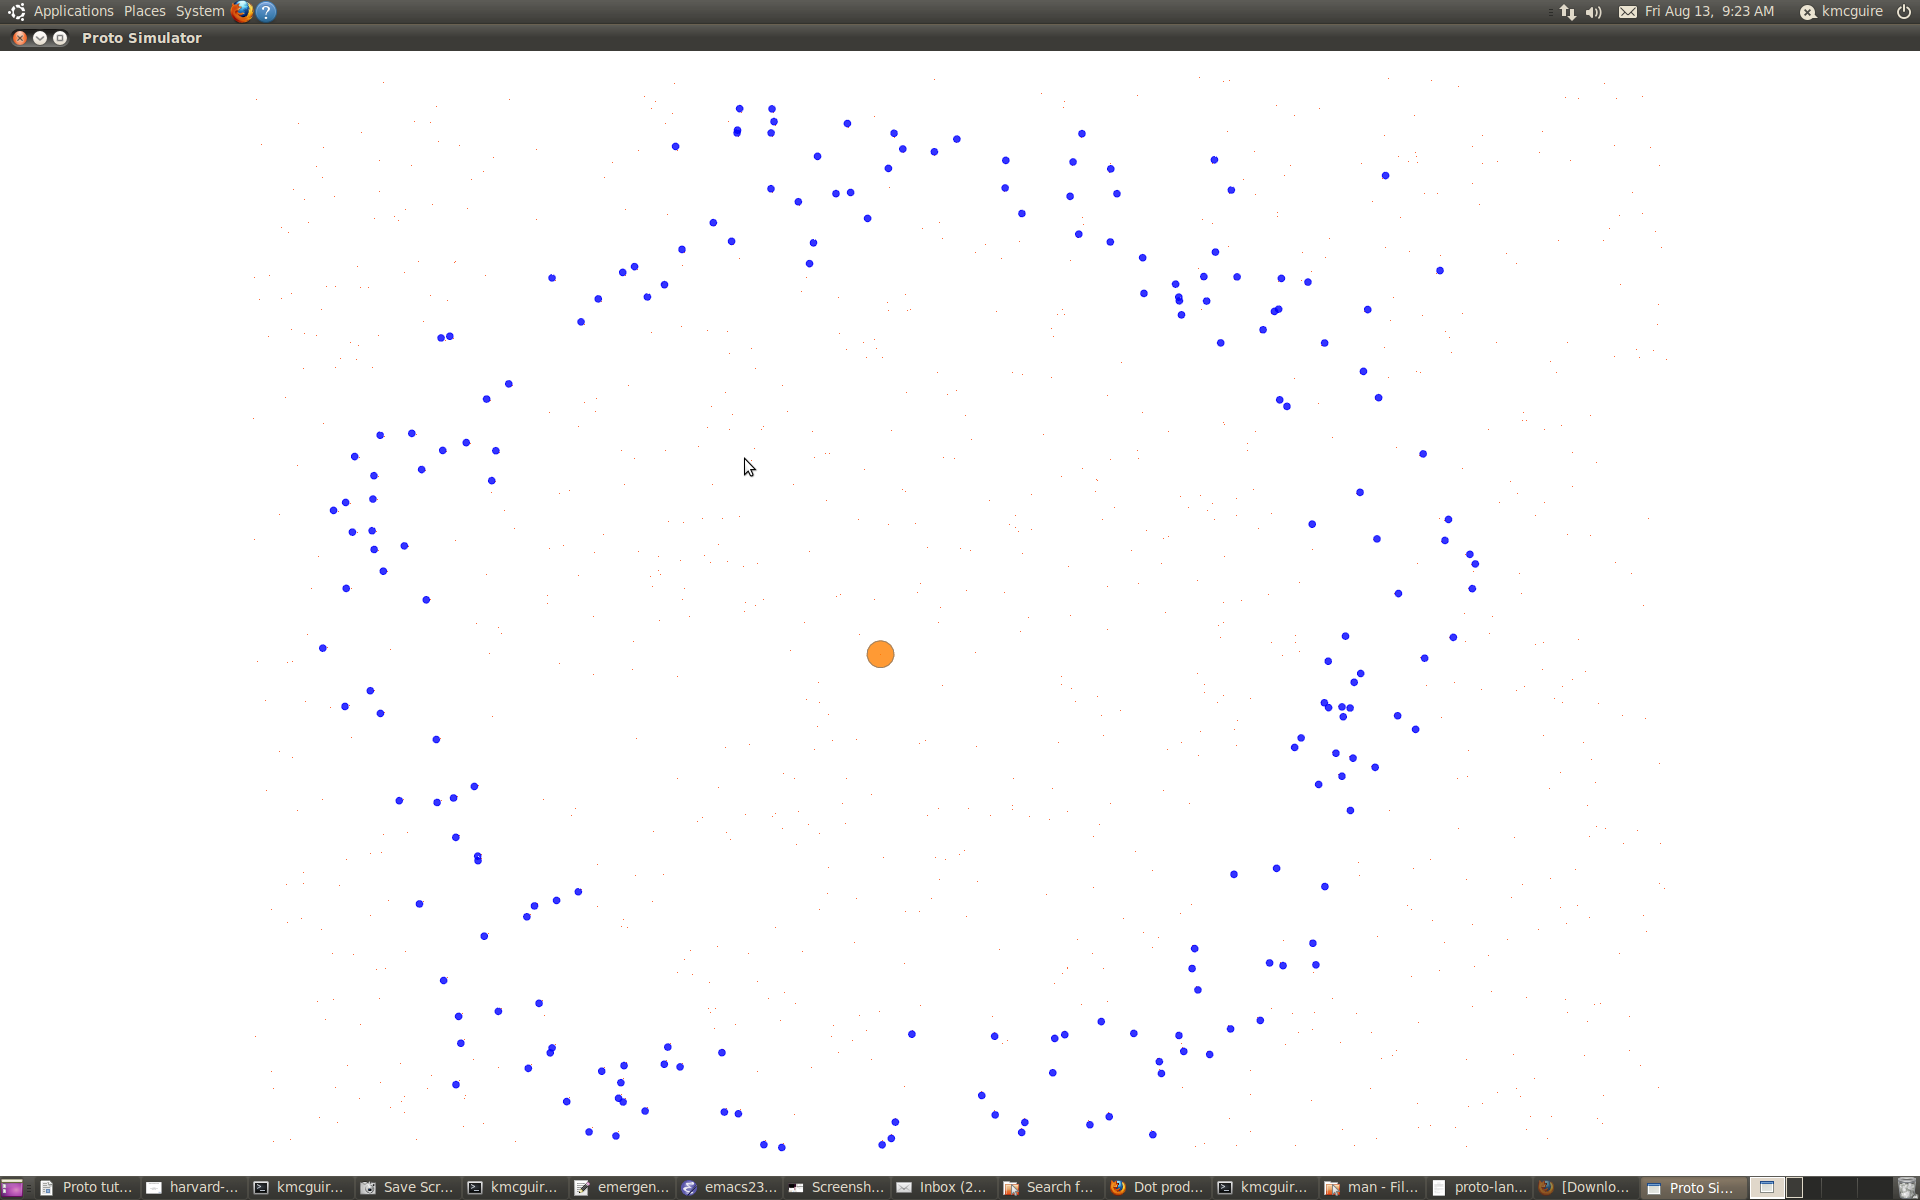
\includegraphics[width=0.38\textwidth]{figures/emergency.png}
  \caption{The \var{emergency} program searching for the farthest device.}
  \vspace{-0.5cm}
  \label{f:emergency}
\end{wrapfigure}

Here, we establish another variable, \var{dis}, as the first value of
\var{d} that is less than infinity.  Now we instead use \var{dis} to
establish \var{max-d} among the devices.  This way we are comparing
the circulating values of \var{max-d} to the original distance
estimated by a device, rather than the alterable values of \var{d}.
This is still a trick, because it is not taking the most accurate
values of \var{d}, but it will at least always choose some device as
the likely farthest.

\problem{Can you come up with a way to always correctly find the
  farthest device using the most accurate values of \var{d}?}

After the farthest device identifies itself, it sets a timer and names
it in the innter \var{let} function.  The timer is now ticking away
invisibly in the farthest device.  Each step, the devices check
whether this timer's value exceeds twenty seconds.  When it does, it
lights its red LED.  Until then, a blue LED is lit. Execute this with
this code in your terminal:

\code{proto -l -n 1000 "(emergency (sense 1))"}

Remember, we use these command line arguments to display LEDs and to
set the number of devices to 1000.  Then turn on \qvar{sense 1} on any
device.  You will soon see blue dots fan out through the points, until
there are just a few dots lit around the edges and in the corners.
Eventually they wink out leaving a single blue dot.  Wait (roughly)
twenty seconds more, and the LED of that device turns red.

This program works fine for the use it is set for, but if you were the
police chief, it is unlikely you would be told you had exactly twenty
seconds to reach an emergency.  You would make that determination
based on what situation you were told was the emergency.  So let's
change this function just slightly.  Instead of setting the time in
the function to an automatic twenty seconds, we will let a value for
time be input into the function from the terminal.  Up to this point
in the tutorial, we have only used a single argument in our functions
(\var{src}), but we are allowed to use as many function arguments as we need.

Let's add the argument \var{TimeTilUrgent}, and change our number of
seconds, 20, to the variable \var{TimeTilUrgent}.  Our function now
looks like this:

\begin{quote}
\begin{verbatim}
(def emergency (src TimeTilUrgent)
  (let* ((d (distance-to src)) (dis (if (< d (inf)) (once d) 0))) 
    (letfed ((max-d 
             0 
             (max (mux (< dis (inf)) dis 0) (max-hood (nbr max-d)))))
      (if (and (< d (inf)) (= max-d dis))
        (let ((timer (rep t 0 (+ t (dt)))))
          (if (>= timer TimeTilUrgent)
              (red 1) 
              (blue 1)))
        0)))) ; Don’t need to do anything: LEDs shut off if not triggered
\end{verbatim}
\end{quote}

When we call the function from our terminal:

\code{proto -l -n 1000 "(emergency (sense 1) 20)"}

The \var{TimeTilUrgent} argument is set again to twenty seconds by
this call, but it can now be set as any numeric value.  We can also
change our timer to measure the progress of something other than
seconds.  For example, it might measure how much fuel is left in an
emergency power generator running at a medical clinic, and we need to
get there before the fuel runs out and leaves the clinic without
power.  If the generator burns 1 gallon of fuel every 5 minutes, then
we can change \var{TimeTilUrgent} into \var{GallonsTilUrgent} and
change \var{dt} to the appropriate fraction of itself: \var{(/ (dt) (*
  5 60))}.  Thus, each second the timer advances by 1/300th of a
gallon, measuring expenditure of 1 gallon every five minutes.  In this
way, we can change the way our timer runs to match the problem that we
are solving.

As the programs used in this section demonstrate, time is a valuable
aspect of Proto.  Play around with the functions you have learned so
far to do a few test programs.  Set a task for the program to perform,
and attempt to reach that goal using your new hold on the Proto
Language.  Remember to use the ever-helpful Proto Language Reference.

\paragraph{Exercises}

\problem{Exercise 1: Modify your microwave timer program to count
  down, like a normal microwave.  Then change the inputs, so that you
  add one minute to the timer every time the user turns \qvar{sense 1}
  on (i.e. if the user toggles \qvar{sense 1} three times, the
  microwave should run for three minutes), and pause the timer
  whenever \qvar{sense 2} is on.}

\problem{Exercise 2: Create a program in which a timer begins in a
  \qvar{sense 1} device.  Red LEDs go on that are within the distance
  of the value of that timer (e.g., when the timer reaches 10 seconds,
  devices within 10 meters from the source turn on red LEDs).}

\problem{Exercise 3: Create a field of 10 points. Have them all turn
  on timers.  If the timer, rounded to the nearest second, is at a
  multiple of three, have it turn its LED red.  If the timer is a
  multiple of three with a remainder of one, turn the LED green.  Else
  turn the LED blue.  Make sure that your program works when the time
  step is fractions, as well as whole seconds.}

\problem{Exercise 4: Write the \var{once} function, which takes in
  an expression and remembers the first value that expression has,
  no matter what it changes to later.}


\section{Using Movement}
\label{s:move}

Because Proto uses a network of numerous devices to perform diverse
tasks, controlling group movement is essential to building for mobile
devices in Proto.  Movement functions may tell devices to move
towards or away from other devices, to follow a leader, to cluster in
groups, and more.  These functions allow users to apply time and
distance functions in new ways with new results. Movement functions
are invaluable to the Proto programmer who wants to use movement in
spatial computing.  Why don't we start by dissecting this example,
which we can call straight out of terminal:

\code{proto -m "(mov (if (sense 1) (tup 3) (disperse)))"}

This program is one of the simplest one can do using Proto
movement. The new parts:
\begin{itemize}
\item \var{tup}: ``tup'' is short for tuple, one of the data types we
  have not used before.  The \var{tup} function takes the values it is
  given and puts them into a short list.  When all of the values are
  numbers, this is a vector, which can specify a speed and
  direction in space.  Generally, the first value this vector is given
  is its length along the x-axis; if it is given a second, that is its
  length along the y-axis.  It can also be given a third for the
  z-axis if we use the 3D mode of the simulator, which will be covered
  later.  Any values we don't put in the vector are assumed to be
  zero.
\item \var{mov}: this function, as shown in the Proto language
  reference, takes a vector and uses it to determine the velocity of a
  device---the speed and direction that the device is traveling.
\item \var{disperse}: this is a separate function that computes a
  vector to each device, so that if the devices follow thei vectors,
  they will move away from other devices within their radio-range.
  This function will vary with different radio-ranges, because the
  devices will only disperse from the devices they are communicating
  with.  Look at page 13 of the Proto Language Reference for more
  information on the \var{disperse} function.
\end{itemize}

Execute this function.  The Proto simulator displays 100 devices.
After a moment, they begin moving about, and you soon have to zoom out
(mouse scroll backwards) in order to see all of them on your screen.
Eventually, they become semi-evenly spaced, wavering just a bit to one
side or the other as they push each other out of communication range.
Now, interrupt this peace by mass-selecting (click and drag over an
area) a group of devices on the left side of the device map.  Then
turn \qvar{sense 1} on for all of these devices.  Keep these devices
selected, without clicking elsewhere.  They all begin to move right
(in the positive direction of the x-axis).  Note that they other
points do not recognize them and move away from them, because we have
used an \var{if} and the \var{disperse} function only effects devices
without \qvar{sense 1}.  \problem{Try coming back later and using \var{mux}
instead to see what happens.}

When these devices are completely in the midst of the other points,
turn \qvar{sense 1} off (if you did not click somewhere else, these
points should still be selected).  The devices around them suddenly
disperse away from them again.

\begin{wrapfigure}{R}{0.4\textwidth}
%  \vspace{-0.8cm}
  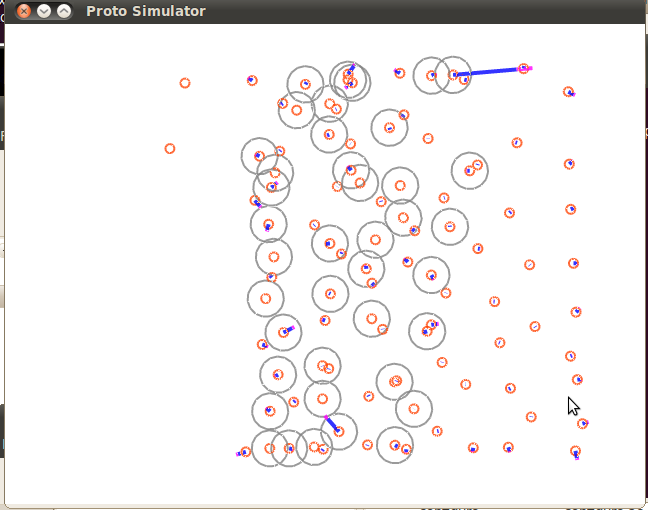
\includegraphics[width=0.38\textwidth]{figures/motion.png}
  \caption{Moving devices dispersing.}
  \vspace{-0.5cm}
  \label{f:motion}
\end{wrapfigure}

Close this program, and then re-execute it.  Turn \qvar{sense 1} on a
few points, and then press ``m'' on your keyboard.  All the devices
are still there, but they have stopped moving.  The ``m'' key toggles
movement on and off from inside the terminal, and as you saw in our
terminal statement, the \qvar{-m} argument there enables movement
initially.  Press ``m'' again to turn movement back on, and then press
``w.''

All the devices that have no doubt strayed outside of their original
placement area now return to fit in the original screen size.  This
argument is very useful because it creates invisible ``walls'' to push
the devices back in to their original distribution area.  You can make
sure the walls are there from the start by adding a \qvar{-w} to the
command line.

Execute this program again (remember, you can simply press the up key
in your terminal to use previous statements).  When the simulator
opens, press the ``v'' key.  The ``v'' key toggles on and off the
display of tuple vectors.  You should now see little blue and pink
tabs on the devices, pointing in the direction of the vectors returned
to the devices.  The larger the magnitude of the vectors the longer
their tuple displays are.  To establish this from the terminal, use
the argument \qvar{-sv}.

Let's try a program that uses both space and motion. Take a look at
this piece of code:

\begin{quote}
\begin{verbatim}
(def MoveIn (src)
  (let ((d (distance-to src)))
    (mux src
         (tup 0 0)
         (let* ((min-d (min-hood+ (nbr d)))
                (vec (int-hood (if (and (< min-d (inf)) (= min-d (nbr d)))
                                   (nbr-vec)
                                   (tup 0 0)))))
           (if (> (vlen vec) 0)
               (norm 0.5 vec) 
               (tup 0 0))))))
\end{verbatim}
\end{quote}

This code is telling all non-source devices to move in towards the
nearest source device.  Well literally, it tells all the neighbors to
move towards whichever of their neighbors is nearest to the source.
Because the source remains stationary, the group is eventually pulled
to congregate on it.  The new parts:
\begin{itemize}
\item \var{let*}: this acts the same way as a normal \var{let}, except
  that adding the \var{*} allows each value to be assigned
  sequentially, so that, values assigned can use variables assigned
  before them in the \var{let*} statement.  In this case, \var{vec}
  uses \var{min-d} in its definition.
\item \var{nbr-vec}: this function returns the field of vectors (x, y,
  z coordinates) to all neighbors within communication distance.
\item \var{int-hood}: takes the integral of the field it is given.
\item \var{norm}: this function tells the device to ignore the
  magnitude of the vector in its second argument (in this case, the
  vectors integrated together in \var{vec}), and just keep the
  direction given, while resetting this magnitude to the first value
  in the \var{norm} function.
\item \var{vlen}: gives the length of a vector.
\end{itemize}

This \var{MoveIn} program is really less complicated than it looks.
First, like in many of our other programs, it finds each device's
distance to the source and names it \var{d}.  Then it asks if any of
the devices are sources.  When one meets this condition, it is told to
remain stationary (but with a \var{mux} so it can still tell others
about its low \var{d} value), while the rest of the points perform the
remaining expressions in the function.  The points then find the
minimum value of \var{d} amongst their neighbors.  In this case,
unlike with \var{closest} back in Section~\ref{s:space}, we're not
looking for the lowest \var{d} anywhere, just amongst our neighbors.

Then, \var{let*} defines the variable \var{vec}, which will tell each
device which direction it should move towards.  This definition takes
the integral, approximated by adding up the vectors from each neighbor
and weighting each by the amount of nearby space that is nearer to
that device than any other.  Inside the integral, the \var{if} asks
each neighbor, is your \var{min-d} less than infinity (this is the
same trick from before, asking if there is indeed a closest point) and
the second part asks each neighbor whether that neighbor has the
lowest \var{d} value (which vector(s) in the field returned by
\var{(nbr d)} equals \var{min-d}).  If devices nearby meet these
qualifications, \var{nbr-vec} takes the vectors to these neighbors,
setting others to zero so that they will not affect the value of the
integral.  Taking the integral (\var{int-hood}) of the selected
\var{nbr-vec} value(s) then assigns \var{vec} as the vector from each
device to the devices with the lowest \var{d} value, which must lie on
the shortest path toward a source device.

After all that, the actual code doesn't really seem like much at all.
The \var{if} asks ``Is the length of your vector greater than 0?;'' in
other words ``have you got a destination that you haven't yet
reached?''  If this is true, and the point still has some way to go,
the device takes the vector it was given, and uses the \var{norm}
function to take away any magnitudes it was given in measuring the
vector, and simply assign the set speed (\var{0.5 meters/second}) in
the direction given in the vector.  If the \var{if} does not return
true, the device is told to stop with \var{(tup 0 0)}.  Ultimately,
this function returns a tuple back to each device, the direction and
speed at which it is to move.

Here is the terminal call:

\code{proto -m -r 30 "(mov (MoveIn (sense 1)))" -s 0.1}

Obviously, because it was only given a tuple by this full function;
our terminal code must tell the devices to move at that velocity using
the \var{mov} function.  This is a common way to do movement in Proto:
calculate the motions for all the devices as vectors, then only at the
very end on the command line send those to \var{mov}.  This makes it
easy to combine movement programs together, since a program can pick
and choose and blend vectors, but commands to \var{mov} don't
blend---only the last one is taken.

We set our source as any point with \qvar{sense 1} on, and then
execute the function.  What about these arguments?  Well, these
arguments tell the simulator to \qvar{-m} (enable movement) and
\qvar{-r 30} (increase communication range to ensure most points are
incorporated).  The \qvar{-s 0.1} tells the simulator that instead of
the default 0.01 simulated seconds per step, we want to run stes of
0.1 simulated seconds.  This speeds up the program (since it redraws
the image ten times less frequently), instead of speeding up the
actual device movement.  Having these devices move too quickly may
cause the group to tear apart. 

\problem{Can you figure out how you would speed them up to find out?
  How fast can you make them go before the program stops working
  correctly?}

Now execute this program.  One hundred red circles appear, randomly
distributed through the simulator space.  Notice they will not move
until the \var{if} statement becomes true with a source device.  Pick
any device, and turn \qvar{sense 1} on.  Instantly all the devices
begin moving towards each other, running into each other and moving
towards the source device.  Before 200 simulated seconds are up, the
devices have been reduced to a wavering red mass inside the orange
circle of your \qvar{sense 1} device.

Let's think about Proto's movement in a new way.  A ship wishes to
sail to its destination.  All we need to do is create a program so a
selected \qvar{sense 1} point (the ship) moves towards a selected
stationary \qvar{sense 2} point (the destination).  That sounds fairly
simple, right?  Just have the ship find out how far and which way to
go, and set it loose.  But this actually leads us to a much more
challenging way of thinking, in which we will separate the movement
from the decision about how to move.  Imagine a field of devices, all
of them displaying their distance to the source.  Illustrate this with
a call in your terminal:

\code{proto -r 10 -s 1 "(distance-to (sense 1))" -v -n 1000}

\begin{wrapfigure}{R}{0.4\textwidth}
%  \vspace{-0.8cm}
  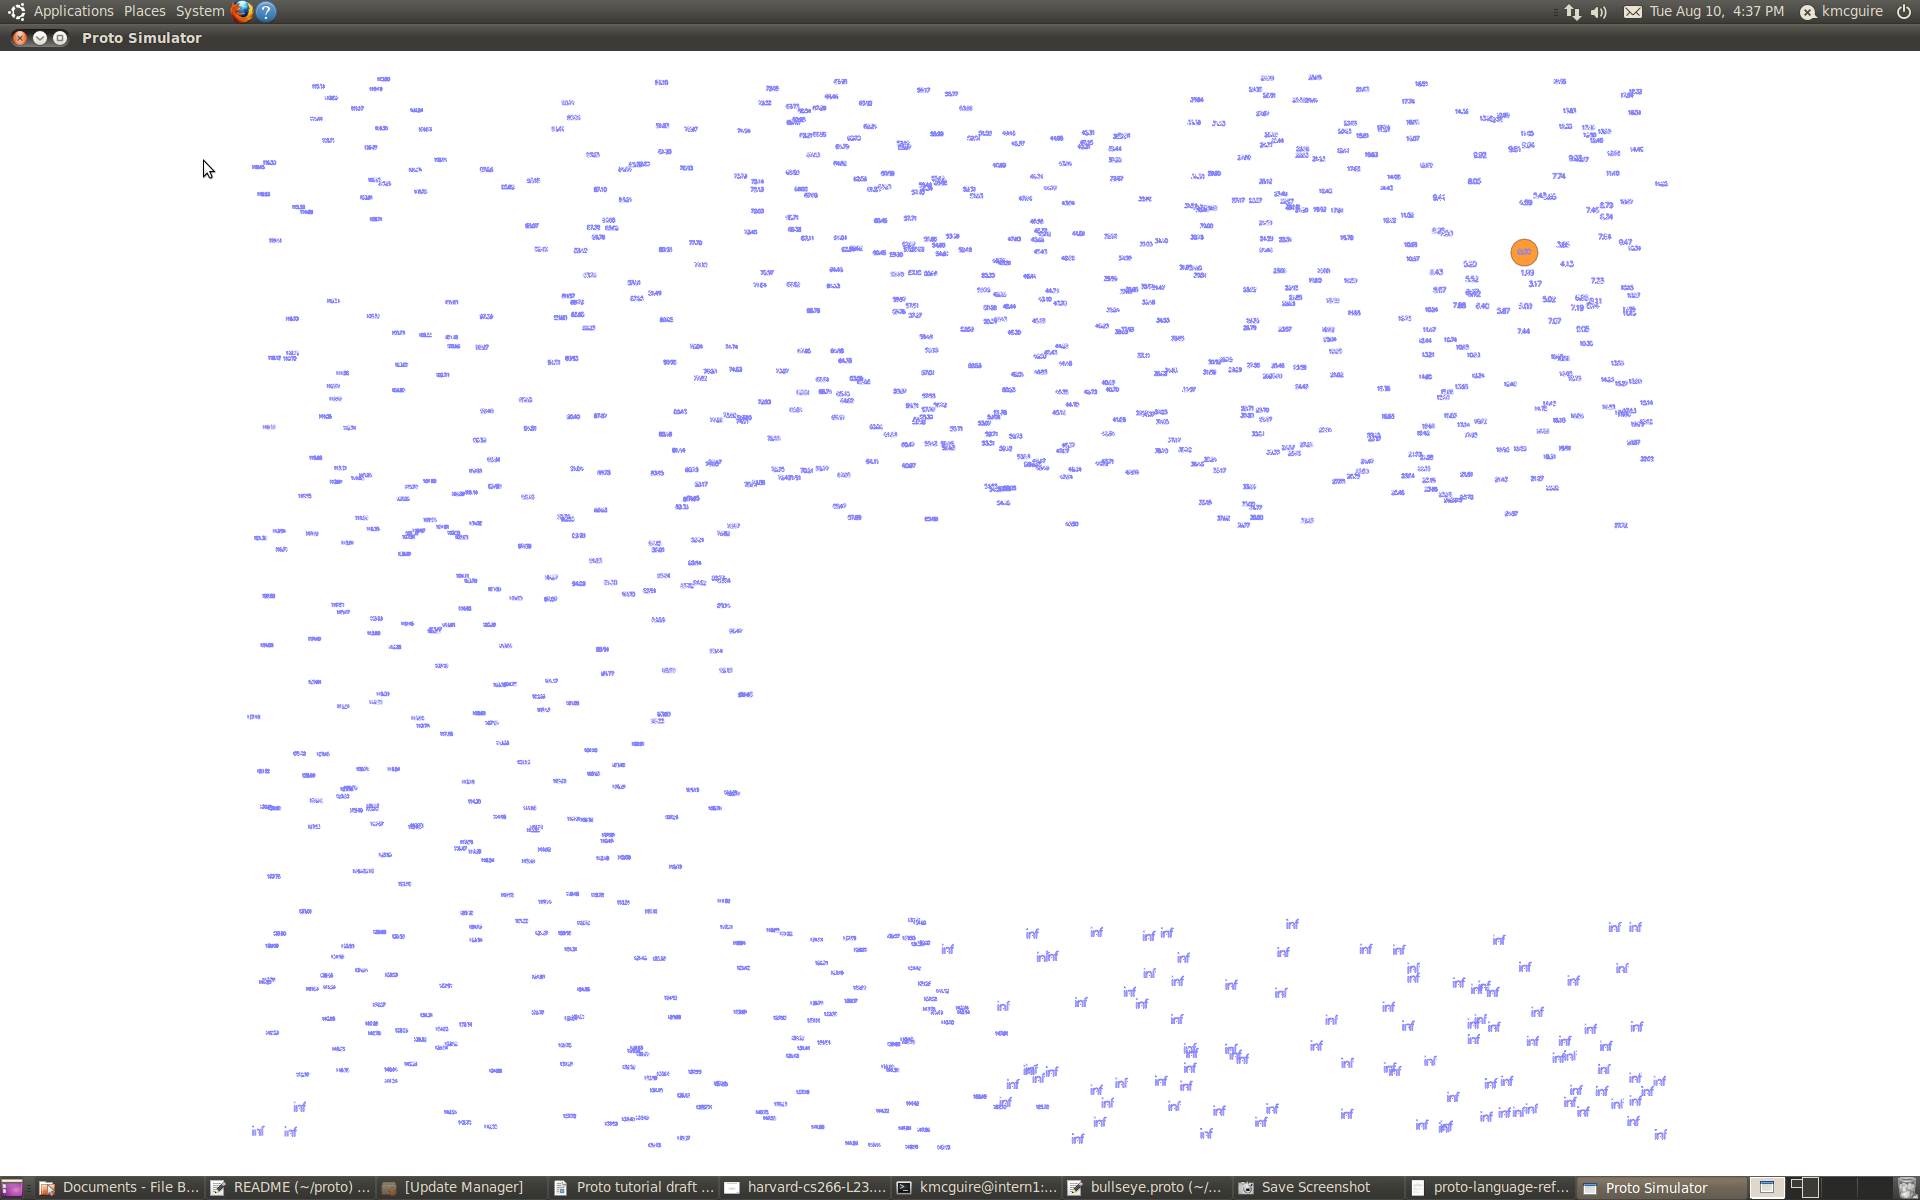
\includegraphics[width=0.38\textwidth]{figures/c-sea.png}
  \caption{A C-shaped ``sea'' of devices}
  \vspace{-0.5cm}
  \label{f:csea}
\end{wrapfigure}

The simulator displays a field full of devices with blue \qvar{inf}
values on top of them.  This code directs all devices to give their
distance to \qvar{sense 1} as their displayed values.  No \qvar{sense
  1} point has been created as of yet, so all their distances are
infinite.  Before you turn on \qvar{sense 1}, select a large amount of
the devices in the middle of the right side. Now move all these points
upward (move with shift-right-click-drag) so that the whole display
looks like a giant ``C'' (a C-shaped sea for sailing).  Now turn
\qvar{sense 1} on at one of the devices at the end of the upper wing
of the ``C.''  All the devices begin to change their values, to
reflect their new distances to the source.  Notice, however, that the
devices' distance values at the end of the lower wing of the ``c'' are
much larger than those in the bottom-left corner.  Because all these
points determine their distances based on the distance values of their
neighbors, these points get their distances by communicating with
their neighbors {\em around} the gap in the ``C,'' rather than over it.
Their distance values are greater because communication is limited by
their shape.  Similar to this, no ocean is perfectly square, so the
ship must follow the shape of the ocean.  Proto allows this easily,
because its values and functions adjust themselves based on the shape
of this ``ocean.''

Now try to visualize this.  Imagine that all the distance values
become heights above the points on the ``C.''  The ``C'' would become
a road-like spiral going downhill, sloping the whole map towards the
source.

In fact, why don't we visualize this in the Proto simulator?  Change
the command line as follows:

\code{proto -r 10 -s 1 "(red (* 0.3 (distance-to (sense 1))))" -l -v -n 1000}

This is the same as before, but turns on LEDs with \qvar{-l} and feeds
the distance values to the red LED after scaling them down so they'll
fit on the screen better.  Make your ``C'' sea as before and turn on
\qvar{sense 1} on an upper right device.  If you rotate the display
around (left-drag with the mouse), you should see something like in
Figure~\ref{f:cdist}.  Remember, you can reset the viewing angle in
the display by pressing ``z.''

\begin{wrapfigure}{L}{0.4\textwidth}
%  \vspace{-0.8cm}
  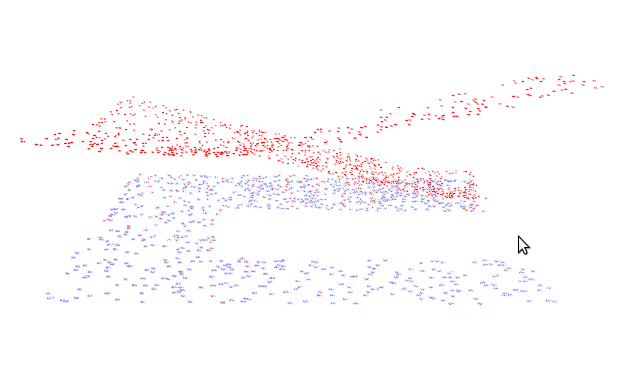
\includegraphics[width=0.38\textwidth]{figures/c-sea-dist.png}
  \caption{Distance to the destination through the ``sea.''}
%  \vspace{-0.5cm}
  \label{f:cdist}
\end{wrapfigure}

Why not use the fact that distances are shaped by the space to our
advantage?  In creating this ship voyaging program, look at it as if
the ship needs to ``roll'' downhill towards the destination, from
greater to lesser distance values.  How do we manage this?

All we need is to have the ship ask the devices within its
neighborhood if their distance values are less than its own.  It can
integrate the vectors to all devices in which this is true, which
averages their directions, but not their magnitudes, and make this its
direction.  This makes it a far more compact program, and we do not
have to worry about communication range because the ship only has to
take into account those devices in its direct neighborhood.  This also
makes it possible for our program to work in more realistic
environments, where we don't have a perfectly square ocean.

Try building this program on your own. Here are some guidelines:
\begin{itemize}
\item Have each device establish its own distance to the destination.
  You will probably want to name this value with a \var{let}.
\item Ask the ship to travel towards the integral (\var{int-hood}) of
  the vectors to neighbors that are closer to the destination than it
  is.  Use the \var{norm} function for the final speed and direction
  of the ship.
\item Tell the destination and all other points to stay put.
\end{itemize}

Remember: \var{mux}s allow for all parts of a program to evaluate and
share information, while the \var{if} only computes the \var{true}
expression in the places where the \var{test} expression is true, or
the \var{false} expression where the \var{test} is false.  Be careful
that where you need your devices to take devices in both branches into
account, you use \var{mux}.  Try to differentiate between these when
writing your program.  Refer to the Proto Language Reference if you
need help.  Consider and refer back to the ``MoveIn'' program, to best
remember how to intertwine space and motion.  When you finish, look
here for our code:

\begin{quote}
\begin{verbatim}
(def voyage (ship destination)
  (let ((d (distance-to destination)))
    (mux destination
         (tup 0 0)
         (mux ship
              (let ((vec (int-hood
                           (if (and (< (nbr d) (inf))
                                    (> d (nbr d)))
                               (nbr-vec)
                               (tup 0 0)))))
                (if (> (vlen vec) 0)
                    (norm 0.2 vec)
                    (tup 0 0)))
              (tup 0 0)))))
\end{verbatim}
\end{quote}

This program establishes \var{d} in every devices as its individual
distance to the source.  Then it asks each device whether it is the
destination.  The destination is instructed not to move with with
\var{(tup 0 0)}.  We use \var{mux} here to make sure that the
destination will participate in the calculation of which way the ship
should go.  Then the program asks whichever devices is the ship
(\var{mux} again for a similar reason) to create a vector (\var{vec}).
This \qvar{vec} is the integral of the field of vectors to neighbors
that meet these conditions: their distances to the source are less
than infinity (to ensure that a destination has been established), and
the ship's distance to the source is greater than theirs.  This way,
the ship now has the vector of the general direction of all the
devices in its neighborhood whose values of \var{d} are less (closer
to the source).  Proto continuously asks if this vector length
(\var{vlen}) is greater than zero (this ship still has some distance
to travel), and if it is, the ship should continue forward at 0.5
meters per second speed, and in the direction of the vector it has
established.

Call this code in your terminal:

\code{proto -m -n 1000 -s 1 "(mov (voyage (sense 1) (sense 2)))"}

This code uses a field with 1000 devices, simulating a large
ocean.  Again, we speed up virtual seconds, this time even faster, so
that the steps run much quicker, but the ship does not have to
increase its speed.  The \qvar{-m}, as expected, allows movement.

Execute this code.  A large field appears full of red circles
representing devices.  Turn \qvar{sense 1} on one point, and
\qvar{sense 2} on another.  Wait a few seconds while the information
is flowing; when neighbor-to-neighbor communication flowing through
the field of devices informs the \qvar{sense 1} point that there is a
destination, it begins moving through the ocean of devices in a
semi-straight line towards the destination.  Within a minute or so, it
reaches and hovers above the destination device.

Close the program, and re-execute it from terminal.  This time, before
turning any \qvar{sense} on, try to create the same gap we created
earlier in this section.  If we put the two \qvar{sense} points each
on the ends of separate wings of the ``C'' shape, you will notice that
the ship device goes all the way around the ``C'' (through the ocean)
to reach its destination, rather than going across the gap.  With
Proto, the programmer is quite able to adapt a program to the
limitations it might have in real life, such as a ship limited by the
shape of its ocean.  Warp the shape of the ocean even more and retry
the program, and watch it navigate any channel as a real ship would.

If you are this far, you now have a fairly good grasp on the movement
aspect of Proto, as well as the space and time branches covered
earlier.  You can probably see how diverse uses for Proto can be, as
it can be applied in numerous real-life situations.  Remember if you
were stumped by this program, or even if you feel like you simply want
a better grasp on any of these functions, they are all defined in the
Proto Language Reference.  Movement, space, and time combine to give
Proto the ability to perform advanced spatial computing tasks.  We
will explore these abilities more in the next section.

\paragraph{Exercises}

\problem{Exercise 1: Adapt the \var{closest} program from
  Section~\ref{s:space}, so that the closest point moves to the
  source.}

\problem{Exercise 2: Adapt the \var{emergency} program so that the
  police device moves to the site of the emergency.}

\problem{Exercise 3: Create a program in which regular points move
  left, \qvar{sense 1} points move right, \qvar{sense 2} points move
  up, and \qvar{sense 3} points move down.}


\section{Advanced Proto}

Now that we have covered the three main aspects, Proto can be taken to
higher levels than so far explained in the tutorial.  We will look at
two complex programs, for flocking and target tracking, then do a 
``graduation test'' problem.

\paragraph{Flocking}
Open the demos folder inside the Proto directory.  Open
\qvar{flock.proto}.  This looks like a big program, but all the text
down at the bottom, where the lines begin with \qvar{;;} are simply
comments letting the reader know about this program.  It is a good
idea to use these comments in your own programs to remind yourself and
others what the objective of the program is.  Also, the programmer has
left a terminal call code (the second comment down), so that one can
easily run this code without having to remember the preferred way to
call it.

What are \var{flock.proto}'s objectives?  It wants all the devices to
arbitrarily group together into flocks of devices following their
neighbors.  Any \qvar{sense 1} devices should travel towards the
middle of the screen, pulling the devices in their groups along with
them.  It becomes a battle between \qvar{sense 1} and non-\qvar{sense
  1} devices to move towards the middle of the screen or ignore the
middle (hence usually moving away).  When there are more than a few
\qvar{sense 1} devices, they will usually win, but sometimes the flock
will tear apart into more than one group.

\var{flock.proto} uses a few new functions:
\begin{itemize}
\item \var{normalize}: this acts in a similar way to the \var{norm}
  function, which we learned earlier, but instead of taking both a
  value and a vector, and setting the length to that of the given
  value, the \var{normalize} function just takes the vector and sets
  the length to one.  Both functions allow the direction of the
  given vector to remain unchanged.
\item \var{vdot}: this operator takes the dot product of the two
  vectors given after it.  The dot product is an algebraic operation
  that takes two coordinate vectors and returns a single number
  obtained by multiplying corresponding entries and adding up those
  products.  For example, two vectors of values [1 0 4] and [3 7 2]
  have a dot product of $(1 * 3 + 0 * 7 + 4 * 2) = 11$.
\item \var{rep}: This is not new, but as we have not used it since the
  beginning of Section~\ref{s:time}.  You are reminded to look it up
  on page 5 of the Proto Language Reference to remind yourself of the
  basic form of a \var{rep} expression.
\end{itemize}

Although these are the only totally new parts, you will find that many
of the things here are used in very different ways than previous
methods.  Let's run through exactly how this function executes.  Looking
at the code:
	
\begin{quote}
\begin{verbatim}
(def flock (dir)
  (rep v
   (tup 0 0 0)
   (let ((d
          (normalize
           (int-hood
            (if (< (nbr-range) 5)
                (* -1 (normalize (nbr-vec)))
                (if (> (nbr-range) 10)
                    (* 0.2 (normalize (nbr-vec)))
                    (normalize (nbr v))))))))
     (normalize
      (+ dir (mux (> (vdot d d) 0) d v))))))
\end{verbatim}
\end{quote}

Before we can really run through this code, we must also know what the
single argument \qvar{dir} holds as its value.  As shown in the
terminal call code, \var{flock} is called with its \var{dir} as this:
\var{(* -0.5 (sense 1) (normalize (coord)))}.  If you look up the
\qvar{coord} part of this, it is not defined in the Proto Language
Reference!  That's because it gives each device a vector of its global
coordinates.  We don't want to assume that is always possible, so
\var{coord} is in one of the optional parts of the simulator
model---see page 14 of the Proto Simulator User Manual.

Imagine a coordinate field.  The middle of the screen is coordinates
$(0, 0)$. A \var{sense 1} device could be in any of the four
quadrants, at any set of coordinates.  The \qvar{(normalize coord)}
part of this statement establishes those coordinates as a direction to
travel.  If a device is at $(x, y)$ on the coordinate plane, what do
we need to do to get it to the origin?  We need to have it travel
$(-x, -y)$.  By multiplying the coordinates of the device by
\var{-0.5}, we tell the device to travel in the opposite direction of
its own coordinates, thereby traveling back to the origin at our newly
set speed of 0.5 meters/second.  Finally, multiplying by \var{(sense
  1)} means that only \qvar{sense 1} devices will move this way: their
value from \qvar{(sense 1)} is 1, while others get 0, which will turn
the whole vector to $(0, 0)$ so they aren't trying to go anywhere in
particular.

This is a primary part of our program.  We have already established
which way \qvar{sense 1} devices want to go.  We feed this into
\var{flock} as an argument, and then continue with the program.  The
\var{flock} program uses the \var{rep} function to evolve the variable
\var{v}. This \var{v} is a vector initialized to 0 (stopped), and then
evolved by the remainder of the function.  We create a variable
\var{d} which establishes the direction in which each device wants to
travel.  The definition adds up influences from each of its neighbors,
which fall into three categories.  Neighbors less than 5 meters away
are ``too close'' and the device moves at a magnitude of one away
(negative direction) from those.  Neighbors that are more than 10
meters away are ``too far'' and the device moves at a magnitude of 0.2
toward them.  Neighbors at an in-between distance (between 5 and 10
meters distant) the device tries to align with, adding in their
\var{v} value.  In this way, devices form groups with their neighbors,
while still keeping a certain distance away.

In the actual function part inside the \var{let}, devices are given a
final direction of \var{dir} (which only matters for sense 1 devices)
plus their values of \var{d}, unless the dot product of \var{d} was
zero (another way of calculating vector length), which generally means
there are no neighbors nearby, so just use the same \var{v} as before.

In the end:
\begin{itemize}
\item Regular points: move away from close neighbors, and towards far
  ones.  Try to move with the direction of the group.
\item Sense 1 points: move towards the middle at strength ``dir,''
  unless the pull of the \var{d} value (the pull from other points),
  is greater.
\end{itemize}

Try executing this program with the call code given in the file.
Remember, when you execute this, we are no longer in your
``MyPrograms'' directory.  You will have to switch to the ``Demos''
directory of the Proto distribution to access this program and call it
from terminal.  Immediately you see a field of purple devices
contorting and moving into clusters.  Now press ``m'' to halt
movement.  The purple was caused by all the blue/red vectors that are
displayed.  Select a large piece of one of the clusters and turn
\qvar{sense 1} on.  Notice that some of the nearby blue devices seem
to blink and adjust their vector display slightly.

\begin{wrapfigure}{R}{0.4\textwidth}
%  \vspace{-0.8cm}
  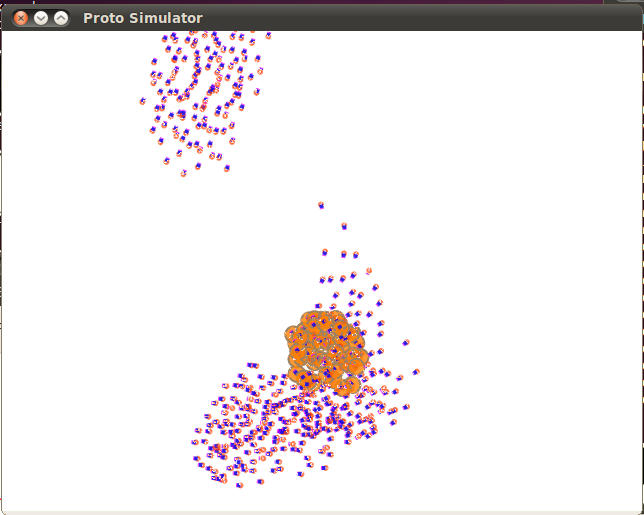
\includegraphics[width=0.38\textwidth]{figures/flock.png}
  \caption{Flocking devices}
%  \vspace{-0.5cm}
  \label{f:flock}
\end{wrapfigure}

Now turn movement back on.  At first it may seem that the groups are
simply continuing to contort, but you will see, if you selected a
large group, the \qvar{sense 1} points tug away from the group,
probably taking a good fraction of the regular points with them, to
``flock'' in the middle of the screen.  The other groups simply
continue on their way.  Try to fool with this program.  Execute it a
few more times, seeing how \qvar{sense 1} points behave when they are
only a small part of the group.  See how a regular point behaves when
it is out of the communication range of all other points.  This
program is designed with the principles of Iain Couzin's 2005 paper on
flock leadership, called ``Effective leadership and decision-making in
animal groups on the move,'' in the journal ``Nature.''

\paragraph{Target Tracking}
Open the \qvar{proto/demos} folder again. Find \var{track-demo.proto}
and open it up.  It may look intimidating, but don't be fooled.  You
know that all the \qvar{;;} lines are comments, and if you look
carefully, there are actually four functions in here, not simply one.
This is because the main function we will look at, \var{track-demo},
calls all the other functions in this file at some point, directly in
itself, or indirectly through another function.  We do not even have
to worry about the first function defined, \qvar{broadcast}, because
we already know what the \var{broadcast} function does.  So scroll
down until you see the line beginning with \qvar{(def channel}; we
will start there.

The function \var{channel}'s purpose is to establish a fat line of
device between the source and the destination devices.  It returns
true for all the points that make up this channel, and false for all
the rest.  Realize that because \var{track-demo} does not take any
arguments, all the functions that it calls (including \var{channel})
must get their arguments from inside it.  Because \var{channel} is
actually called in \var{track}, which is itself called by
\var{track-demo}, we must follow first the arguments given to
\var{track} in \var{track-demo}, and then what arguments these create
in \var{channel}.  If we define all the arguments used in all
functions:
\begin{itemize}
\item \var{target} in \var{track} is any \qvar{sense 1} device
\item \var{dst} in \var{track} is any \qvar{sense 2} device
\item \var{coord} in \var{track} is the coordinates of devices
\item \var{src} in \var{channel} is any \var{sense 1} device
\item \var{dst} in \var{channel} is any \qvar{sense 2} device
\item \var{width} in \var{channel} is 10
\end{itemize}

Okay, so \var{channel} establishes \var{d} as the distance between the
source and the destination.  Then it establishes \var{trail} as a
boolean (true or false) variable where each device asks: Is my
distance to the source plus my distance to the destination, less than
or equal to their distance between each other plus one meter?  If this
is true, they are on the shortest path between the source and the
destination.  If our distance numbers were perfectly accurate, we
wouldn't have the ``plus one,'' but they aren't, and the extra bit
makes sure we get a trail.

Finally, \var{channel} returns true for all devices in which \var{d}
is less than infinity (ensuring that a destination and a source have
been established), and which fit the dilated \var{width} of the
trail. This \var{dilate} function simply takes the given devices---in
this case our shortest-path \var{trail}---and expands it to include
any devices that are within the given \var{width}. The \var{width}
given to this call of \var{dilate} is ten, so any devices ten meters
or less from the \var{trail} become part of the channel.

Now switch to the \var{track} function.  This takes all its arguments
from the list above as well.  Remember that the \var{all} function
simply runs through all the expressions it is given in parallel.  The
function still returns the value of the last expression that it is
given.  First, \var{track} restricts to run on only the points
returned as true from the \var{channel} function.  Then these devices
turn their LEDs blue, and the \var{dst} device computes the distance
between its own coordinates and the coordinates of the \var{target},
which are \var{broadcast} to it through the channel (remember that the
\var{broadcast} is running only inside the channel because we are
using \var{if}).  The other points simply return (tup 0 0 0).

Lastly, the \var{track-demo} function.  This uses the \var{all}
function again, and also two other functions:
\begin{itemize}
\item \var{rnd}: this is simply a function that chooses a random
  number between the two numbers that follow it.  In this case, it
  picks a random number between 0 and 1.
\item \var{once}: recall from Section~\ref{s:mux} that this computes
  the expression after it only once and then remembers it.
\end{itemize}

This function first establishes the true or false boolean variable
\qvar{mobile}, which has a 50/50 chance of being true, and stays that
way because of the \qvar{once}.  Then the next statement tells the
devices to move if they are a \qvar{sense 1} devices or a \qvar{sense
  2} device, or if \var{mobile} is true (approximately half of the
devices).  Then they move at 0.01 magnitude of the vectors returned by
the \qvar{dither} function, which results in slow movement in a random
direction.  Finally, also perform the track function.  Note that the
track function simply returns a tuple to the target at the
destination, which is displayed but does not moved with.

Execute this program with the last terminal code listed in the
\var{track-demo.proto} file.  Again, remember that you will need to be
in the \var{proto/demos} directory in you terminal to execute this.
Turn on \qvar{sense 1} on one point, and \qvar{sense 2} on another.
You will see blue dots fan out from the target and destination, then
link up and suddenly a vector display forms linking the two.  Half the
points will float around (dither), including these two, but they will
remain connected by this tuple display.


\paragraph{Graduation Test}

Okay, now you are probably pretty handy at Proto, so let's try one
last programming test.  This one uses time, space and movement
together.  Here is the situation:

There is an Olympic runner, who is up for the race of her lifetime.
The lowest time of the day is on the board.  If she can beat it, she
wins the gold medal.  Build a function that takes several arguments
(speed, time, runner, start, and finish) to help you simulate how fast
she will need to go.  Execute this program with the runner as
\qvar{sense 1}, the start line as \qvar{sense 2}, and the finish line
as \qvar{sense 3}.  When ready to execute, input the best time
currently on the boards (you may choose this).  When executing the
program, you will want \qvar{sense 1} to approach the starting line,
and then stop.  When the finish line is turned on, have both the timer
start and the runner begin running.  If the runner reaches the finish
line before the timer is up, turn on a green LED on the runner.  If
she does not reach it in time, stop him, and turn on a red LED
instead.  Adjust the runner's speed and the distance between the start
and finish until you have the runner win a narrow victory.

Hint: the \var{letfed} and \var{broadcast} functions will prove
helpful in this program.  Look them up in the Proto Language Reference
for help.  Also, look at your previous ``ship voyage'' program.  Using
this may simplify the movement part of your program significantly.
When you think you have it, look here for our code:

\begin{quote}
\begin{verbatim}
(def olympian (speed time runner start finish) 
  (letfed ((t 0 (if finish (+ t (dt)) 0))) 
    (if (= (broadcast finish t) 0) 
        (mov (goto speed runner start)) 
        (if (< (broadcast finish t) time) 
            (let ((d (distance-to finish))) 
              (if (and runner (< d 1)) 
                  (mov (tup 0 0 0)) 
                  (mov (goto speed runner finish))))
            (tup 0 0 0)))
    ; first 'paragraph' deals with motion vectors

    (let ((d (distance-to finish))) 
      (if (and runner (< d 1)) 
          (green 1) 
          (if (< (broadcast finish t) time) 
              0
              (if runner (red 1) 0))))
    ; second 'paragraph' deals with LEDs
    ))
\end{verbatim}
\end{quote}

Now, our code actually uses a sub-functions for this project, as you
will see if you look closely and find the \var{goto} function that is
hidden in there.  This is not a function we have simply not covered,
but a function we wrote specifically for use in this program.  A large
part of our \var{olympian} function was simply moving one point to
another (runner to start and runner to finish), so we pulled this out
as a separate new \var{goto} function, and then called it inside of
the \var{olympian} function instead of putting all of its code there
twice.  Here is our \var{goto} function.

\begin{quote}
\begin{verbatim}
(def goto (speed mover destination)
 (let ((d (distance-to destination)))
   (mux destination
        (tup 0 0 0)
        (mux mover
             (let* ((vec (int-hood 
                           (if (and (< (nbr d) (inf)) 
                                    (> d (nbr d)))
                               (nbr-vec)
                               (tup 0 0 0)))))
               (if (> (vlen vec) 0) 
                   (norm speed vec)
                   (tup 0 0 0)))
             (tup 0 0 0)))))
\end{verbatim}
\end{quote}

Looking over this, you may notice that it is almost entirely identical
to the \var{voyage} function that we created in the
Section~\ref{s:move} of this tutorial.  The only differences, in fact,
are that we added a speed argument so that we may choose the speed of
motion when we call the function, and changed the \qvar{ship} variable
name to a more generic \qvar{mover}.  By using this \var{goto}
function, as with the \var{voyage} program, the runner will follow an
indirect path to the finish line.  The user of this program can now
set an actual track down for the runner to follow to the finish line,
rather than simply cutting through on a straight line to the finish
line.

Knowing this \var{goto} function, let's look at the \var{olympian}
program and figure out how it works.  It begins by starting a
\var{letfed} timer, which evolves only inside the finish line device.
Remember, the \var{letfed} timer works much like the \var{rep} timer,
but instead of just returning the variable \var{t}, it makes it
available for use by the rest of the program.  In this case, we
establish this \var{t} to always be zero except in the finish line
device.

Next we see what looks like two separate ``paragraphs'' of code, with
spaces in between.  Both of these pieces of code are actually running
at once.  These parts cannot easily be combined into one block of
nested \var{if}s, because they return different data types.  The first
part deals with movement and therefore tuple data types, and the
second deals with LEDs, which return scalar (real number) values.

The first part asks whether the value of \var{t} being broadcast from
the finish device is zero (there is not yet a finish line, so the race
has not begun).  If it is zero, then have the runner \qvar{goto} the
start.  Remember that the \var{goto} function returns a vector, so we
must tell the device to move at that velocity with the \var{mov}
function.  If this value of \var{t} broadcast from the finish is not
zero (the race has begun), we want the runner to \var{goto} the finish
line, but only if she has not yet reached the finish line, and if the
timer has not yet exceeded the lowest time, which we input into the
function as \qvar{time}.  The \var{if} statement here checks whether
the timer has yet exceed time, and if it has the runner needs to stop.
If it hasn't, the next \var{if} checks whether or not the runner is
within one meter from the finish line (essentially there), and if the
runner is, it is again told to stop.  If you used a zero value there,
it is highly unlikely that the runner will ever reach exactly zero,
and it will more likely waver over the finish line indefinitely.
Otherwise, the runner continues to go towards the finish line until
one or the other of these checks become true.

The second part is relatively simple. We simply ask again those same
two questions: ``Have I reached the finish line?'' and ``If not, has
the timer exceeded the input value of time?.''  If the first question
is true, turn the LED green, otherwise if the second question is true,
turn the LED red.  In all other cases, keep the LED off.  Try running
\var{olympian} with this call in your terminal:

\code{proto -m -s 1 -l -c "(olympian 0.2 500 (sense 1) (sense 2) (sense 3))"}

\begin{wrapfigure}{R}{0.4\textwidth}
%  \vspace{-0.8cm}
  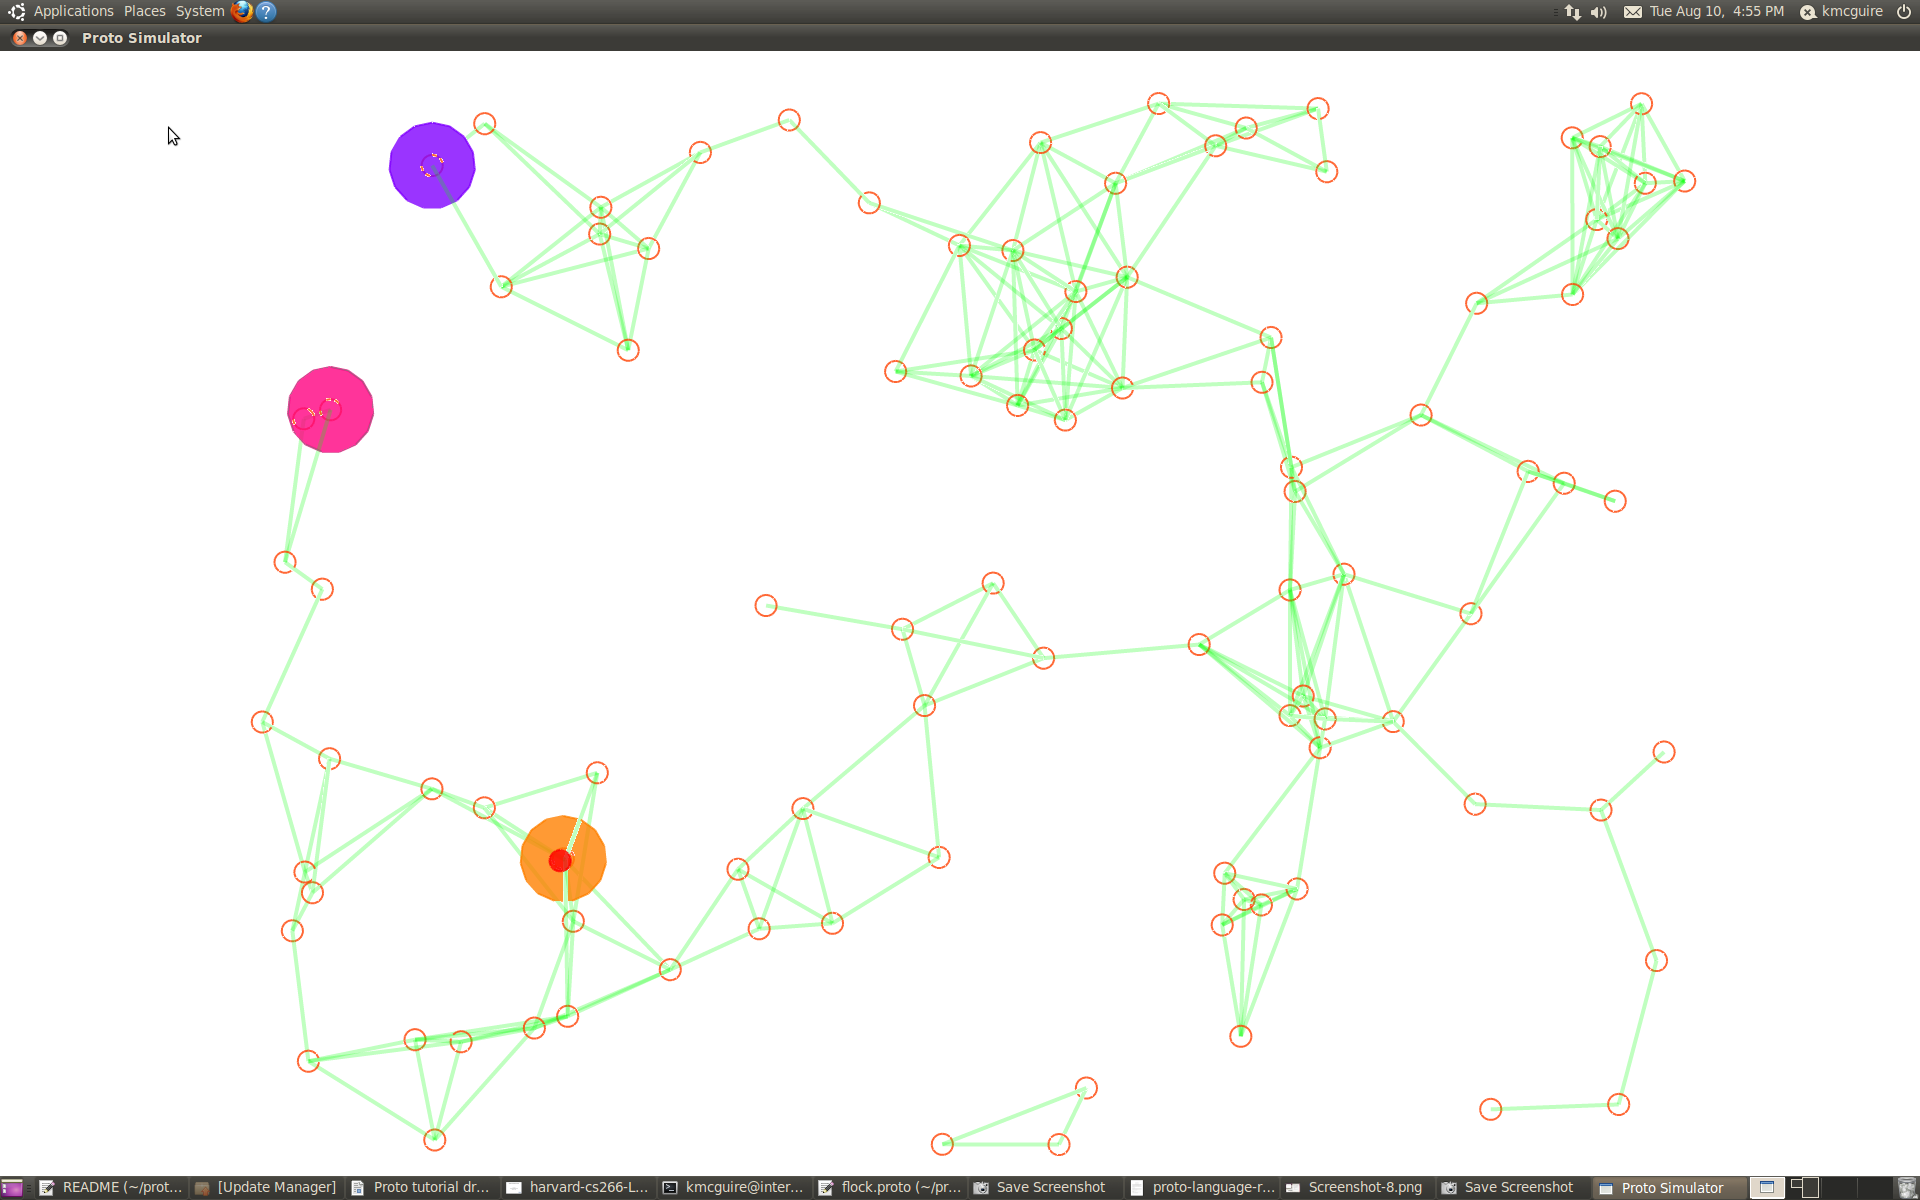
\includegraphics[width=0.38\textwidth]{figures/olympian-lose.png}
  \caption{The \var{olympian} loses a race.}
%  \vspace{-0.5cm}
  \label{f:olympianloes}
\end{wrapfigure}

Before you execute this, look at some of the values we have put in as
the variables. We have set our speed to 0.2 meters/second, and also
sped up the simulation step size with the \qvar{-s 1} command.  We
have set the time of the fastest runner on the board so far as 500
simulated seconds, and enabled movement, LEDs and visible network
connections.  The runner, start line, and finish line have been set to
their respective senses.

\begin{wrapfigure}{R}{0.4\textwidth}
%  \vspace{-0.8cm}
  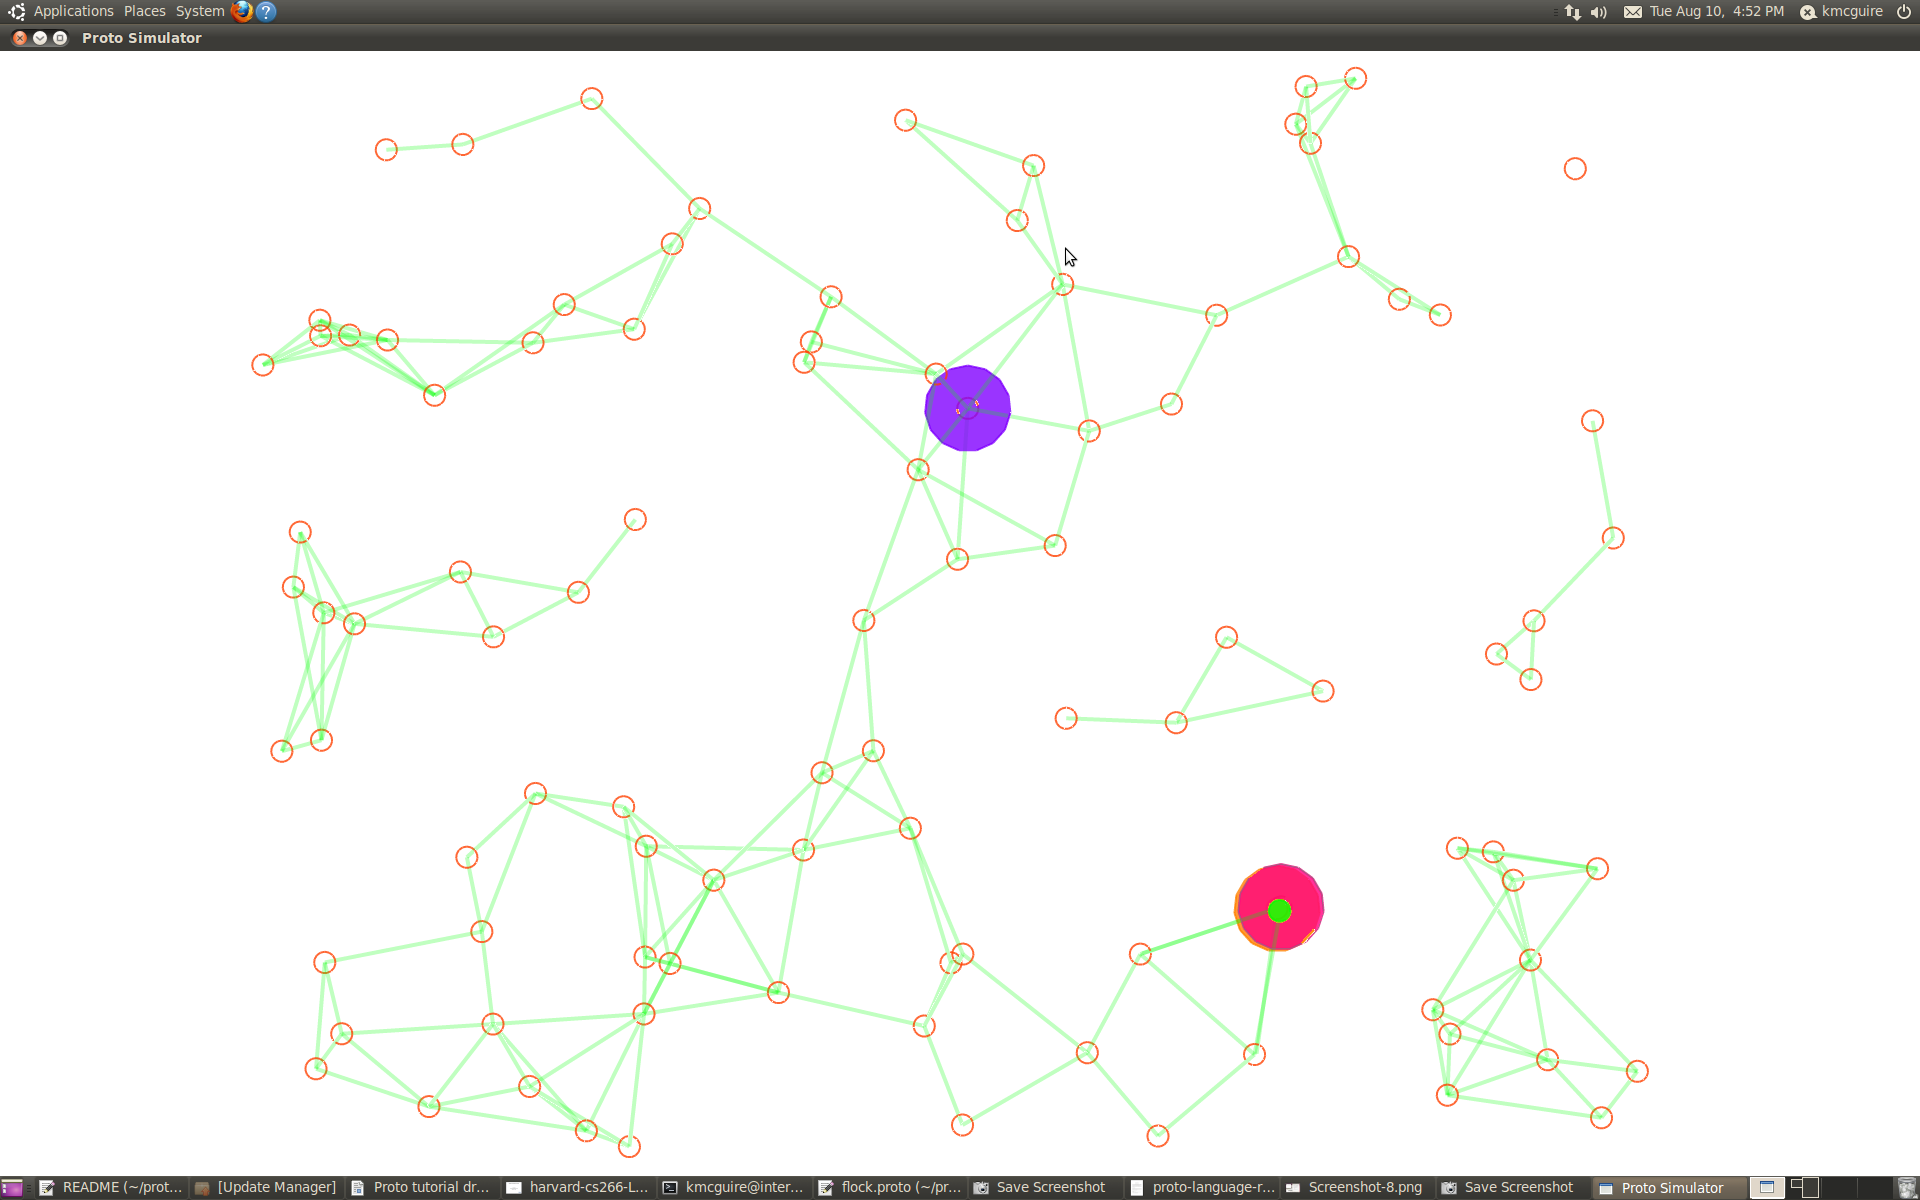
\includegraphics[width=0.38\textwidth]{figures/olympian-win.png}
  \caption{The \var{olympian} wins a race.}
%  \vspace{-0.5cm}
  \label{f:olympianwin}
\end{wrapfigure}

Execute this call in terminal. You should see an interestingly
structured web of green connections and little red circles.  You may
either simply take the large and messy route in front of you as the
runner's ``track,'' or create one yourself by moving around the
points.  Make sure the track that you want to use is all connected.
Pick any point connected to the track (which will not break any major
connections by moving), and set it as the runner (\qvar{sense 1}).
Then set a point as the start line (\qvar{sense 2}), and watch as the
runner makes its way over to the start.  When the runner has reached
the start line, set a finish line to kick off the race.  If they are
connected, the runner will soon begin to make its way to the finish,
at the set speed of 0.2 meters/second.  Depending on how far away your
start and finish lines are, the runner will either stop and turn its
LED red, or go all the way to the finish line and turn its LED green,
winning the race.

Re-execute this program, and change the inputs for speed and time in
your terminal.  Change the distance and the ``track'' in the
simulator.  See how this effects the outcome of the race.  Try the
race with only ten devices and set up a small, clearly formed track
for the runner to follow.

Now, let me give you a new idea. In this program, and the demo ones
that we looked at, you may have wondered why the tup values had three
0's rather than just two.  Proto, along with the many other things it
can do, can take its simulation to the literal next dimension.  These
zeros become the x, y and z coordinates of a 3D coordinate plane.  Try
the same \var{olympian} program call, adding a \qvar{-3d} argument to
the terminal call code.  Also, extend the range to 40, and get rid of
the \qvar{-c} argument to stop the connection display.  Execute this.

\begin{wrapfigure}{R}{0.4\textwidth}
%  \vspace{-0.8cm}
  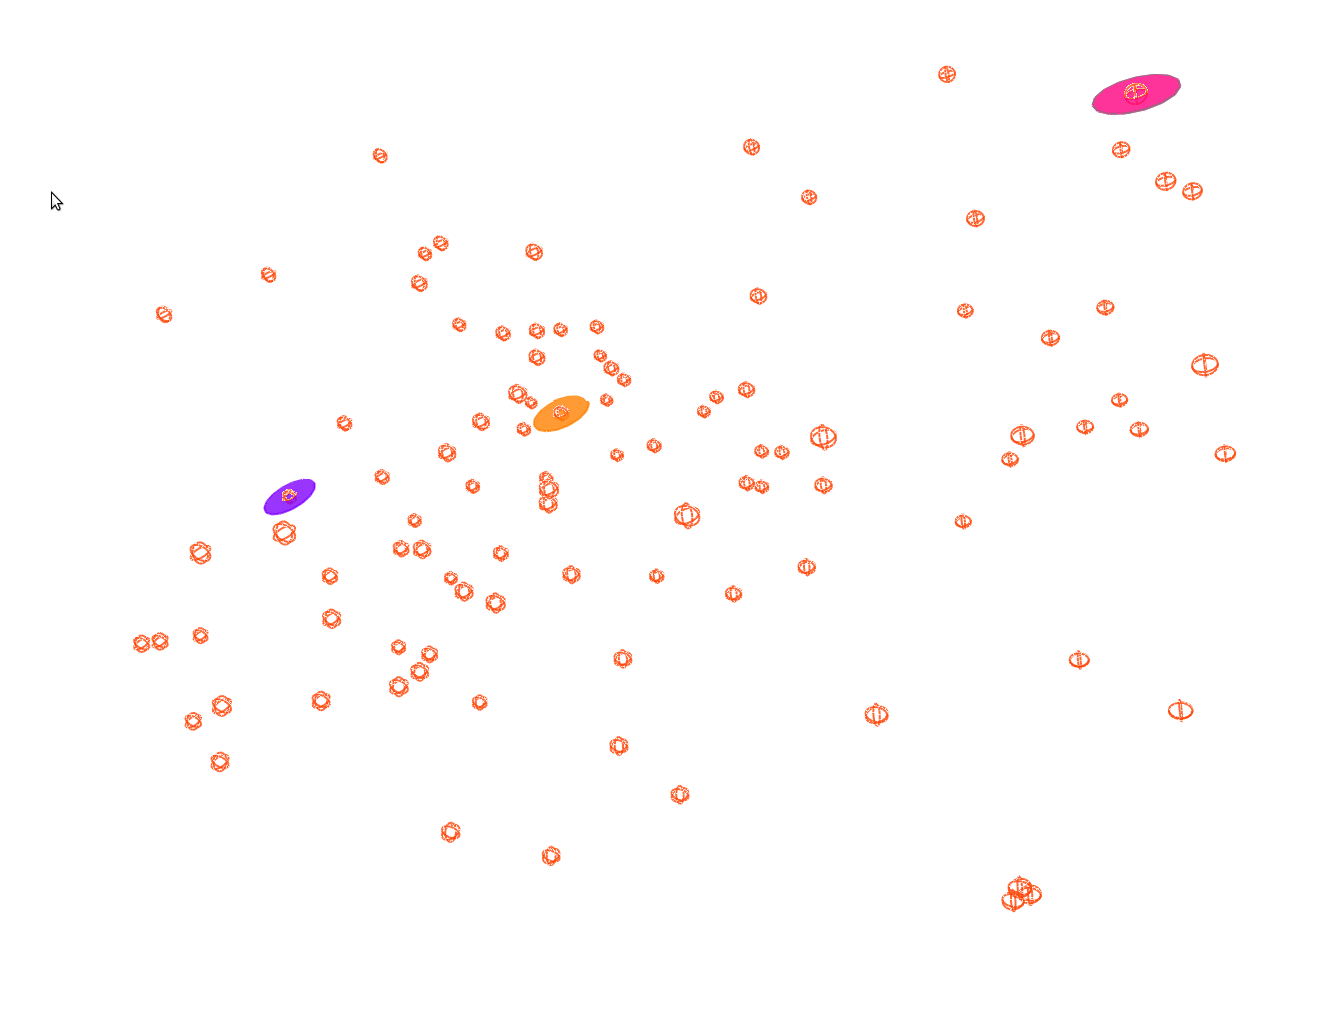
\includegraphics[width=0.38\textwidth]{figures/olympian-3d.png}
  \caption{The \var{olympian} runs a 3D race.}
%  \vspace{-0.5cm}
  \label{f:olympianthreed}
\end{wrapfigure}

You should now see the regular field of 100 devices, but this time the
little circles are spheres instead, and are all different sizes.  This
is because some of them are farther away than others.  Left-click-drag
to rotate the field of view and see the box-like collection of devices
from other angles.  If you turn the senses on as you would normally in
this program, the runner will actually run at different heights within
the box to get to a finish line on a totally different
plane. 

\problem{Challenge: Go back to the MoveIn program, and make it run in
  3d mode.}

\paragraph{Exercises}
\problem{Exercise 1: Go back to the examples and programs you
  struggled with. Try them again with your new understanding.}

\problem{Exercise 2: Right now the \var{flock} program tells the Proto
  simulator to change the flocks movement based on three even sections
  of the default communication range of fifteen meters (within 5
  meters, above 10 meters, and in between).  Adjust this so it takes
  three even sections of any given communication range.}

\problem{Exercise 3: Adjust the \var{olympian} program so that the
  finish and start lines are established as actual lines (between two
  points), and so that multiple runners can run, one after another.
  (Multiple runners can run currently, but after a finish line has
  been established they no longer take the start line into account).}

\problem{Exercise 4: Change the \var{olympian} program so that it
  detects when a runner has {\em crossed} the finish line rather than
  when a runner has reached it.}

\problem{Exercise 5: Create a 3D ``pool'' in which someone is diving
  for treasure.  Have one device at the top of the ocean dive for a
  stationary device at the bottom, and then have the diver bring the
  ``treasure'' back to the top with it.  Set a timer to make sure the
  diver doesn't run out of air, and light an LED when it is close to
  running out.}

\problem{Exercise 6: Imagine some other real-life situation (some
  ideas: bowling, animals foraging for food, someone parting a crowd
  as he walks).  Apply Proto to model it.}

If you have made it to this point, and you are pretty confident in the
programs you have read and built, you have grasped how to think in
Proto.  Congratulations!  We encourage you to take Proto further with
some exploits of your own, and remember to use the Proto Language
Reference for any of the functions we have not explained in this
tutorial.  Hopefully you now, like us, also think that Proto is an
extremely useful and easy way to program spatial computers.

\end{document}